 %%%%%%%%%%%%%%%%%%%%%%%%%%%%%%%%%%%%%%%%%
% OIST Doctoral Thesis - Temporary bound version
% LaTeX Template
% Version 0.2 (2016/04/06)
%
% This version is the temporary binding version which will be submitted to the thesis examiners.
% Many features (such as double spacing) are meant for the examiners' convenience, do not modify them.
%
% Original author:
% Jeremie Gillet
%
%%%%%%%%%%%%%%%%%%%%%%%%%%%%%%%%%%%%%%%%%

%-------------------------------------------------------------------------------
%	PACKAGES AND OTHER DOCUMENT CONFIGURATIONS (do not modify)
%-------------------------------------------------------------------------------

\documentclass[12pt, oneside]{book} % 12 pt font, one-sided book style
\usepackage[a4paper, includehead, headheight=0.6cm, inner=2.5cm ,outer=2.5cm, top=2.5 cm, bottom=2.5cm]{geometry}  % Changing size of document
\usepackage[english]{babel} % The document is in English
\usepackage[utf8]{inputenc} % UTF8 encoding
\usepackage[T1]{fontenc} % Font encoding

\usepackage{graphicx} % For including images
\graphicspath{{./Images/}} % Specifies the directory where pictures are stored

\usepackage{longtable} % tables that can span several pages
\usepackage{setspace} % For using double spacing
\usepackage[bf, font=onehalfspacing]{caption} % caption: FIG in bold, 1.5 line spacing in figure and table captions
\usepackage{pdfpages} % If you want to include a pdf file of your published paper as an appendix

\usepackage{fancyhdr} % For the headers
\usepackage{braket}

\newcommand{\numberedchapter}{ % Preparation for numbered chapters
	\cleardoublepage % To make sure the previous headers are passed
	\lhead{\bfseries \leftmark}}% Header
\newcommand{\unnumberedchapter}[1]{ % Preparation for unnumbered chapters
	\cleardoublepage % To make sure the previous headers are passed
	\phantomsection % To help hyperref link to the right page
	\addcontentsline{toc}{chapter}{#1} % Also adds the chapter name to the Contents
	\lhead{\bfseries #1}}% Header

\usepackage{eso-pic} % For the background picture on the title page
\newcommand\BackgroundPic{%
\put(-260,-140){%
\parbox[b][\paperheight]{\paperwidth}{%
\vfill
\centering
\includegraphics[width=\paperwidth]{symbol.jpg}%
\vfill
}}}

\usepackage{hyperref} % Adds clickable links at references

%-------------------------------------------------------------------------------
%	CUSTOM VALUES, COMMANDS AND PACKAGES (NOT IN THIS FILE)
%-------------------------------------------------------------------------------

% Open Preamble/mydefinitions.tex and enter some values (name, thesis title...)
% also include your own custom LaTeX functions and packages
% DO NOT add your packages here to ensure the temporary and final thesis use the same packages

%-------------------------------------------------------------------------------
%	VALUES FOR THE THESIS
%-------------------------------------------------------------------------------

\newcommand{\name}{James Schloss} % Author name
\newcommand{\thesistitle}{Advanced split-operator techniques for simulating quantum systems} % Title of the thesis
\newcommand{\submissiondate}{July, 2019} % Submission date "Month, year"
\newcommand{\supervisor}{Thomas Busch} % Supervisor name
%\newcommand{\cosupervisor}{C.~O'Supervisor} % Co-Supervisor name, comment this line if there is none


%-------------------------------------------------------------------------------
%	BIBLIOGRAPHY STYLE (pick the style you want)
%-------------------------------------------------------------------------------

\usepackage[square, numbers, sort&compress]{natbib} % for bibliography - Square brackets, citing references with numbers, citations sorted by appearance in the text and compressed (as in [4-7])
%\usepackage[longnamesfirst,round]{natbib} % Natural Sciences bibliography

%\bibliographystyle{Preamble/physics_bibstyle} % You may use a different style adapted to your field
\bibliographystyle{abbrvnat} % You may use a different style adapted to your field


%-------------------------------------------------------------------------------
%	YOUR PACKAGES (be careful of package interaction)
%-------------------------------------------------------------------------------

\usepackage{amsthm,amsmath,amssymb,amsfonts,bbm}% Math symbols

%-------------------------------------------------------------------------------
%	YOUR DEFINITIONS AND COMMANDS
%-------------------------------------------------------------------------------

% New Commands
\newcommand{\bea}{\begin{eqnarray}} % Shortcut for equation arrays
\newcommand{\eea}{\end{eqnarray}}
\newcommand{\e}[1]{\times 10^{#1}}  % Powers of 10 notation

% Defining a theorem box for Criteria
\newtheorem{critere}{Criterion}
\newcommand{\crit}[2]{
\begin{center}  
\fbox{ \begin{minipage}[c]{0.9 \textwidth}
\begin{critere}
\textbf{\textup{ #1}} --- #2
\end{critere}
\end{minipage}  } \end{center}
}


\begin{document}

%-------------------------------------------------------------------------------
%	TITLE PAGE
%-------------------------------------------------------------------------------

\pagestyle{empty} % No page numbers
\frontmatter % Use roman page numbering style (i, ii, iii, iv...) for the preamble pages

\begin{titlepage}
\AddToShipoutPicture*{\BackgroundPic}
\begin{center}
\vfill
{\large \scshape Okinawa Institute of Science and Technology\\Graduate University}\\[0.7cm]
{\large Thesis submitted for the degree }\\[0.7cm]
{\Large Doctor of Philosophy}\\[0.5cm]
\rule{\textwidth}{1.5pt}\\[0.5cm]
{\huge \bfseries \thesistitle}\\[0.5cm]
\rule{\textwidth}{1.5pt}\\[2.5cm]
\hfill  by\\[1cm]
\hfill  {\large \bfseries\name}\\
\vfill
{\hfill \large Supervisor: \textbf{\supervisor}} \\
\ifx\cosupervisor\undefined\else{\hfill \large Co-Supervisor: \textbf{\cosupervisor}} \\ \fi
\vspace{1cm}
\hfill  \submissiondate
\end{center}
\end{titlepage}

%-------------------------------------------------------------------------------
%	PREAMBLE PAGES (delete unnecessary pages)
%-------------------------------------------------------------------------------

\pagestyle{fancy} % Change the header style
\fancyhf{}% Clear header and footer
\renewcommand{\chaptermark}[1]{\markboth{#1}{}} % Getting the chapter name right
\rhead{\thepage} % Page number at the right of the header
\frontmatter % Use roman page numbering style (i, ii, iii, iv...) for the preamble pages
\setcounter{page}{2} % Include the title page in page counting
\doublespacing % Double spacing

\unnumberedchapter{Declaration of Original and Sole Authorship} 
\chapter*{Declaration of Original and Sole Authorship} 

I, \name, declare that this thesis entitled \emph{\thesistitle} and the data presented in it are original and my own work. 


I confirm that:
\begin{itemize}
\item No part of this work has previously been submitted for a degree at this or any other university.
\item References to the work of others have been clearly acknowledged. Quotations from the work of others have been clearly indicated, and attributed to them.
\item In cases where others have contributed to part of this work, such contribution has been clearly acknowledged and distinguished from my own work.
\item None of this work has been previously published elsewhere, with the exception of the following: 
\begin{itemize}
\item Chapter~\ref{ch:1d} is largely derived from a paper published in the New Journal of Physics (\textbf{18}(3):035012, 2016)~\cite{schloss2016}.
\item Chapter~\ref{ch:2d} is largely derived from a paper published in Phys. Rev. Fluids (\textbf{4}(5):054701, 2019)~\cite{zhang2019}.
\item The GPUE codebase, which is a primary topic in Chapter~\ref{ch:gpu} has been published in the Journal of Open Source Software (\textbf{3}(32):1037, 2018)~\cite{schloss2018}.
\item Chapter~\ref{ch:vortex_states} is largely derived from a recently submitted manuscript to Phys. Rev. Fluids (arXiv:1910.02364)~\cite{schloss2019}.
In addition, many figures for this chapter have been created for the GPUE documentation~\cite{docs}.
\item Figure~\ref{fig:bench} was created by Peter Wittek when comparing different numerical solvers~\cite{wittek2016}.
\item Figure~\ref{fig:expr_tree} was largely derived from tikz code provided by Xadisten during a Twitch livestream.
\item Figure~\ref{fig:coalesce} was largely derived from tikz code created by user Realz Slaw on stackexchange~\cite{stackoverflow}.
\item Figure~\ref{fig:mode_plot} was Reproduced by Nieddu \textit{et al.} and Kumar \textit{et al.}~\cite{Nieddu2016, kumar2015}.
\end{itemize}
All of the articles mentioned above have been (or will be published) under Creative Commons BY with attribution to the original authors, and in each chapter, I clearly define my focus in each publication.
\end{itemize}

Date:  \submissiondate

Signature: 





\unnumberedchapter{Abstract} 
\chapter*{Abstract} 
\subsection*{\thesistitle}

The split-step Fourier method is a powerful technique for solving partial differential equations and simulating quantum systems of various forms. In this body of work, we focus on several variations of this method to allow for simulations of one, two, and three-dimensional quantum systems, along with several notable methods for controlling quantum systems, including quantum optimal control and shortcuts to adiabaticity. We also examine the creation of stable, three-dimensional vortex structures in Bose--Einstein condensates through rotation, artificial magnetic fields, and phase imprinting, and we analyze chaotic vortex trajectories in two dimensions. In addition, we discuss algorithmic optimizations for implementing the compressed split-step Fourier method for graphics processing units and multicomponent simulations. All features present in this work have been incorporated into a state-of-the-art and open-source software suite known as GPUE and are justified with physical systems where such techniques have been applied.

\unnumberedchapter{Acknowledgment} 
\chapter*{Acknowledgment}

Firstly, I would like to acknowledge the work of my advisor, Thomas Busch.
His tireless effort to help his students pursue their best interests is honestly inspiring.
I greatly appreciate his kindness, honesty, and willingness to try new things.
I would also like to acknowledge the work of my online community, the Algorithm Archivists, as they constantly motivated me to learn new methods for my research.
This work has been supported by the Okinawa Institute of Science and Technology (OIST) Graduate University and used the computing resources of the Scientific Computing and Data Analysis section.
This work has also been supported by JSPS KAKENHI JP17J01488.
I would also like to thank (in no particular order) Lee, Mossy, Angela, Albert, J\'er\'emie, Peter, Irina, Ben, Tiantian, Peter (2), Rashi, Valentin, Ankur, the Quantum Systems Unit, and the OIST community for being such wonderful people and helping to varying degrees throughout my time at OIST.
Finally, I would like to thank Ayaka for helping me focus on something other than work for a change.

\input{Preamble/abbreviations}
\input{Preamble/glossary}
\input{Preamble/nomenclature}
\input{Preamble/dedication}

%-------------------------------------------------------------------------------
%	LIST OF CONTENTS/FIGURES/TABLES
%-------------------------------------------------------------------------------

\unnumberedchapter{Contents}
\tableofcontents % Write out the Table of Contents
\unnumberedchapter{List of Figures}
\listoffigures % Write out the List of Figures
\unnumberedchapter{List of Tables}
\listoftables % Write out the List of Tables

%-------------------------------------------------------------------------------
%	THESIS MAIN TEXT
%-------------------------------------------------------------------------------

\addtocontents{toc}{\vspace{2em}} % Add a gap in the Contents, for aesthetics
\mainmatter % Begin numeric (1,2,3...) page numbering

\unnumberedchapter{Introduction} % Title of the unnumbered chapter
\section*{Introduction}
The Split-Step Fourier Method (SSFM) is an essential technique for simulating a variety of physical systems and is particularly useful for simulating the propagation of wave packets for single and multimode fibers~\cite{agrawal2000, sinkin2003, meirelles2005, min2003} and various quantum systems~\cite{bayindir2015, weideman1986, wang2005}, including all simulations performed in this work.
Though other methods, such as explicit and implicit Euler~\cite{butcher2016}, Crank-Nicholson~\cite{crank1947}, and Runge-Kutta~\cite{butcher2016}, can solve similar differential equations, the SSFM has distinct advantages over these methods.
For example, the SSFM is often much easier to parallelize than Runge-Kutta~\cite{brehler2017}, as it primarily relies on embarrassingly parallel element-wise matrix multiplications and Fast Fourier Transform (FFT) routines that have been optimized for parallel and distributed systems.
The SSFM also provides a lower error bound than either the Euler or Crank-Nicholson methods, and does not require implicit or tridiagonal solver \cite{conte2017, thomas1949} which are also not easily parallelizable~\cite{goddeke2010, wang1981, sweet1977}.
A full discussion of the advantages and disadvantages of the SSFM can be found in Chapter~\ref{ch:splitop}.

For the purposes of this text, we will be focusing on the application of the SSFM to quantum systems and will use primarily physical arguments to understand the details of the method, itself.
We will also discuss several numerical techniques for optimally simulating quanum systems on massively parallel Graphics Processing Units (GPUs), along with software developed for this purpose: GPUE, the Graphics Processing Unit Gross-Pitaevskii Equation Solver.
This work will discuss several additional areas of interest for implementing similar solvers on GPUs, including distributed transposes and important considerations for traditional FFT routines for simulating quantum systems on multiple GPU devices.

As such, it is important to first discuss several principles of quantum systems in Chapter~\ref{ch:qs}, incuding the Schr\"odinger equation which governs the dynamics for simple quantum systems along with several notable variations that correspond to physical systems to be discussed in this work.
Further elaboration on advances in scientific computing, including the massively parallel Graphics Processing Unit (GPU) will be discussed in Chapter~\ref{ch:gpu}, and the SSFM method, along with variations on the method for vortex simulations will be discussed in Chapter~\ref{ch:splitop}.
In Chapter~\ref{ch:1d}, we will discuss the basics of quantum engineering, by generating macroscopic superposition states of highly-interacting quantum particles with quantum optimal control and shortcuts to adiabaticity.
In Chapter~\ref{ch:dynamics}, we will discuss specifically superfluid simulations and several notable methods for generating and controlling vortex structures both theoretically and experimentally, along with numerical hurdles with simulating such systems on GPU architecture, and in Chapter~\ref{ch:2d}, we will discuss an application of the GPUE codebase in the generation of chaotic vortex dynamics with a small number of vortices in a two-dimensional superfluid simulation.
In Chapter~\ref{ch:3d}, we will discuss challenges in simulating fully 3-dimensional, multi-component superfluid systems on GPU architecture, including dynamic field generation, storage limitations, and spectral methods to optimize the simulation, itself.
In Chapter~\ref{ch:vortex_states}, we will apply the numerical techniques introduced in this text to simulate a novel device that couples the evanescent field of an optical nanofiber to generate vortex ring-like structures in a toroidally trapped superfluid system.
Finally, we will conclude by discussing key results from this work, along with future directions in both theoretical and computational physics.
 % Introduction (unnumbered)

\chapter{Introduction to the split-operator method} \label{ch-splitop}

 % Introduction (unnumbered)

\numberedchapter % Regular chapters following

\chapter{Introduction to GPUE codebase and General Purpose computing with Graphical Processing Units (GPGPU)} \label{ch-gpu}

% I don't think acronyms should be defined in titles --- ABC

\section{General purpose computing with graphics processing units}
\section{Special considerations for the GPUE codebase}
 % Input your chapters here
\chapter{Engineering NOON states in one-dimensional quantum gases}
\label{ch:1d}

Until recently, simulating dynamic control protocols to engineer specific quantum states have been difficult to perform on GPU devices without full control of the software, itself.
This meant that researchers wishing to engineer specific quantum states by using GPU simulations would be required to have domain-specific knowledge in both software design and quantum mechanics, neither of which are trivial to understand.
This chapter serves as motivation for several methods to be discussed in Chapter~\ref{ch:gpu} to allow for the simulation of quantum control methods on GPU devices, with a particular focus on quantum optimal control~\cite{werschnik2007} and Shortcuts To Adiabaticity (STA)~\cite{guery2019}.
Both of these control protocols will be used in a physical example for the non-adiabatic generation of superposition states in a one-dimensional Tonks--Girardeau (TG) gas~\cite{schloss2016}.
To start, I will discuss the field of optimization algorithms before moving to STA protocols and a physical system using both in practice.

The work in this chapter has been published in \textit{New Journal of Physics}~\cite{schloss2016}, and in this publication, I performed all calculations for all the figures generated and focused primarily on optimal control methods.
The STA protocol was devised by J\'er\'emie Gillet, and the research was supervised by Albert Benseny and Thomas Busch.

\section{Optimization methods}

Optimization algorithms have become essential to many areas of modern computing and focus on either minimizing or maximizing a cost function by modifying several control parameters~\cite{lewis2012}.
The number of control parameters create an $n$-dimensional space to traverse, and optimization algorithms are tasked at finding the global minimum or maximum of this domain.
For certain domains, it is difficult to find a global optimization strategy and many methods instead get caught in local minima while attempting to find the appropriate solution.
Because generalized optimization is such a fundamental problem, there are many known optimal control methods, such as gradient descent~\cite{ruder2016}, the Nelder--Mead or simplex method~\cite{nelder1965}, genetic algorithms~\cite{koza1997}, and many more~\cite{lewis2012}.
Of these, gradient descent is often considered to be one of the easiest to implement with favorable complexity and convergence guarantees, and because of this, it has become ubiquitous in many areas such as machine learning, which is of particular interest for GPU engineering. 
Even so, there are limitations to gradient descent, such as its dependence on calculating the gradient of the cost function's solution domain along with lengthy convergence times for high-precision solutions.

For this work, I am primarily interested in the area of quantum optimal control, which is a method typically used to determine the optimal time-dependent control parameters necessary to transform an initial state to a final, desired state~\cite{werschnik2007}.
This means that one will often be maximizing the fidelity between states, defined as $\mathcal{F} = |\braket{\psi|\phi}|^2$, where $\psi$ is the engineered quantum state and $\phi$ is the state one is attempting to replicate.
This problem can be re-framed as an attempt to find the maximum of a fidelity \textit{landscape}, where each point in the domain is a calculation of the fidelity.
This means that each point in the fidelity landscape necessarily involves solving the Schr\"odinger equation for chosen control parameters.
For this reason, I will be introducing a gradient-less (derivative-free) optimization algorithm, the Nelder--Mead (simplex) method, which is often used as a heuristic approach to this problem and there are several known optimizations for this method~\cite{nelder1965,kolda2003,lewis2007}.
The Nelder--Mead method is also the recommended optimization algorithm for the chosen quantum optimal control method of the physical example that will be discussed in Section~\ref{sec:CRAB}, Chopped RAndom Basis (CRAB) optimal control.

\subsection{Nelder--Mead}
\label{sec:NM}

The Nelder--Mead method is one of the most commonly implemented gradient-less optimization algorithms to-date and relies heavily on the concept of a simplex, which is a generalization of the three-dimensional tetrahedron to $n$-dimensions.
For example, a 0-simplex is a point, a 1-simplex is a line, a 2-simplex is a triangle, a 3-simplex is a tetrahedron, and so on.
If the Nelder--Mead method is attempting to optimize a cost function with $n$ control parameters, an $n+1$ point simplex will be created, and the points of this simplex will be manipulated until they have converged to a minimum or maximum in the domain.
For this section, I will focus on the method introduced in the original work by Nelder and Mead in 1965 while working at the National Vegetable Research Station in Warwick, England~\cite{nelder1965}.

For $P_i \in i=\{0,...,n\}$ simplex points with heights of $y_i \in i=\{0,...,n\}$, the Nelder--Mead method is tasked at minimizing all points such that $\sqrt{\sum(y_i-\bar y)^2/n} < \eta$, where $\bar y$ denotes the height of the centroid location of the simplex, and $\eta$ is some pre-defined convergence threshold value.
This convergence criteria assumes that if all points have converged with this method, the final location must be the minimum of the optimization domain; however, as mentioned in the previous section, this method may become trapped in a local minimum.
At every step in the Nelder--Mead method, the points with the highest and lowest values are determined and denoted as $P_h$ and $P_l$, respectively.
In addition, the centroid location is found as $\bar P$.
This method then performs up to three basic operations on the simplex, itself:

\begin{description}

\item[Reflection] For this operation, $P_h$ is flipped across $\bar P$, such that the new location,
\begin{equation}
P^* = (1+\alpha)\bar P - \alpha P_h.
\end{equation}
\noindent Here, $\alpha > 0$ is a constant known as the reflection coefficient.
After this operation, the new height is compared to $y_l$.
If it is lower, the method proceeds to an expansion step.
Otherwise, the method checks whether the new height is lower than some other $y_i \in \{0,...,n\},n\neq \{l,h\}$, and if it is, the point is kept and the method continues to find the new simplex ordering.
If it is found that the reflected point, $P^*$, is higher in value than all other points, the method then keeps whichever point corresponds to the lowest height between the reflected and previous highest point and proceeds to the contraction step.

\item[Expansion] For this operation, an expansion is performed, such that the new location,
\begin{equation}
P^{**} = \gamma P^* + (1-\gamma)\bar P.
\end{equation}
\noindent Here, $\gamma > 1$ is a constant known as the expansion coefficient.
If the new height is less than the previously lowest point, the expanded point, $P^{**}$, is kept, otherwise the reflected point is kept.

\item[Contraction] For this operation, a contraction is performed, such that the new location,
\begin{equation}
P^{**} = \beta P_h + (1-\beta)\bar P.
\end{equation}
\noindent Here, $0 < \beta < 1$ is a constant known as the contraction coefficient.
If the contracted point, $P^{**}$, is lower than the previous highest point, the contracted point is kept, otherwise, the entire simplex is contracted closer to the lowest point with $P_i = (P_i + P_l)/2$.
\end{description}

Each step in the Nelder--Mead method begins with a proposed reflection of the least optimal point about its centroid position.
From there, the method follows the protocol described above.
The choice of $\alpha$, $\beta$, and $\gamma$ is somewhat arbitrary and should be optimized by-hand.
An example of the centroid locations for minimization using this method with the Rosenbrock banana function~\cite{pohlheim2007} can be seen in Figure~\ref{fig:minimize_NM}.

\begin{figure}
\center 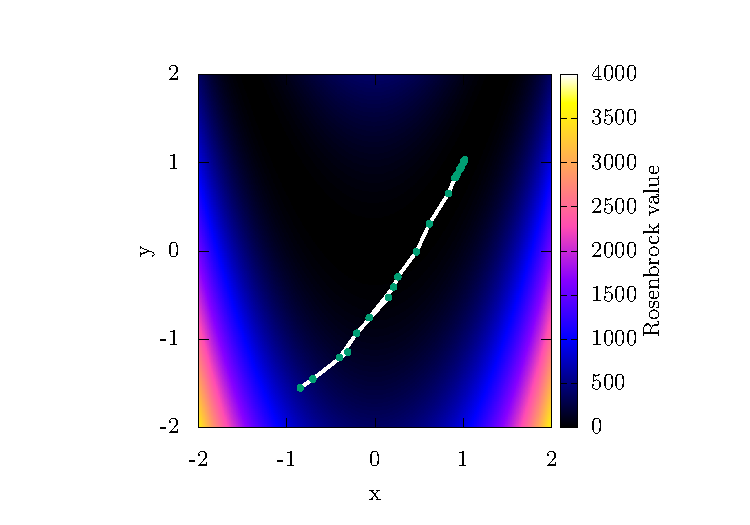
\includegraphics[width=0.75\textwidth]{data/1d/NM/NM.pdf}
\caption{Plot of the centroid locations (green dots connected with white line) for the Nelder--Mead method while optimizing the Rosenbrock banana function, $f(x,y)=(a-x)^2+b(y-x^2)^2$, with $a=1$ and $b=100$.
Here, centroid locations start at $(-0.851,-1.553)$ and end at the known minimum of $(1,1)$ in 19 iterations.
Here, $\alpha = 1$, $\beta = 0.5$, and $\gamma = 1.5$.}
\label{fig:minimize_NM}
\end{figure}

Even though the Nelder--Mead method is a heuristic approach and can become stuck in a local minimum, as long as a sufficient number of random simplexes are chosen at the start of the simulation, it can be used to find an adequately optimal solution.
Ultimately, any gradient-less optimization algorithm can be used to traverse the fidelity landscape for quantum optimal control, and in the next section, I will discuss a common method used in the field: the CRAB optimal control method.

\subsection{Chopped random basis optimal control}
\label{sec:CRAB}

The CRAB technique works by modifying a control parameter for a given system, $\Gamma$, with a multiplicative term as
\begin{equation}
\Gamma^{\text{CRAB}}(t) = \Gamma^0(t)\gamma(t),
\end{equation}

\noindent where $\Gamma^0(t)$ is an initial guess, and the function $\gamma(t)$ is written as a sum of $2J$ sinusoidal functions,
\begin{equation}
\gamma(t)=1+\frac{1}{\lambda(t)}\sum_{j=1}^J(A_j \sin(\nu_jt) + B_j\cos(\nu_jt)).
\end{equation}

\noindent Here, $\lambda(t)$ is usually defined by the system, such that $\Gamma^{\text{CRAB}}$ and $\Gamma^0$ coincide at initial and final times.
This means that $\lim_{t\rightarrow 0} \lambda(t) = \lim_{t\rightarrow T}\lambda(t) = \infty$, where $T$ is the final time of evolution.
As such, any smooth function may be chosen with these constraints.
For example, one might use
\begin{equation}
\lambda(t) = \frac{T^2}{4t(t-T)},
\end{equation}
\noindent which satisfies the provided conditions.
This then transforms the optimal control problem into an optimization of the space spanning $\{A_j, B_j, \nu_j\}$, which can be done by using Nelder--Mead with a simplex of random initial points.
As an example, if $J = 10$, a thirty-dimensional space would be created and a thirty-one simplex would be formed to traverse this space.
It is important to remember that each new simplex and simplex-operation requires re-solving the Schr\"odinger equation for those values, and as such, this is a computational costly technique.
Even though higher $J$ values will produce a more accurate result, lower values should be chosen, if possible.

This method is a general-purpose computational tool for determining the optimal pulse to ensure the generated state is as close to the desired state as possible, and I will show an example of it being used later in this chapter.
Even so, it is sometimes worthwhile to attempt to devise analytical frameworks that serve a similar purpose, and for certain systems, this can be done with STA protocols.

\section{Shortcuts to adiabaticity}

STA protocols are semi-analytical methods that allow for quantum state generation while retaining the effects of adiabatic movement.
Here, adiabatic processes are defined as actions by which slow changes in the control parameters leave particular properties invariant, such as the quantum number~\cite{guery2019}.
The ultimate goal of STA protocols is to achieve adiabatic motion in sub-adiabatic time, and this can be done in a number of ways; however, in this section, I will introduce only the invariant-based inverse-engineering approach using Lewis--Riesenfeld invariants~\cite{torrontegui2013}.
In particular, I will focus on the specific methods necessary for the example to be introduced later in this chapter and much of this section will follow traditional derivations from various sources~\cite{torrontegui2013,guery2019, schloss2016}.

With the method of Lewis-Riesenfeld invariants, the theory for relating different eigenstates of a time-dependent, Hermitian invariant to the solutions to the Schr\"odinger equation~\cite{lewis1969} can be applied to systems with time-dependent Hamiltonians, such that
\begin{equation}
i\hbar \frac{\partial I(t)}{\partial t} - \left[\mathcal{\hat H},I(t)\right] = 0,
\end{equation}
\noindent where $I(t)$ is the invariant.
This ensures that the expectation values for the states driven by $\mathcal{\hat H}$ are constant in time.
It is possible to expand the state of the system $\ket{\Psi(t)}$ into the orthonormal basis of the invariant with,
\begin{equation}
\ket{\Psi(t)} =\sum_{n=1}^\infty c_n e^{i\alpha_n(t)} \ket{\phi_n(t)},
\end{equation}
\noindent where $c_n$ are time-independent amplitudes for each state, and $\ket{\phi_n(t)}$ are orthonormal eigenvectors of the invariant, such that
\begin{equation}
I(t) = \sum_n^\infty\ket{\phi_n(t)}\lambda_n\bra{\phi_n(t)}.
\end{equation}
\noindent Here, the $\lambda_n$ are real constants, and the phase is defined as ~\cite{lewis1969}
\begin{equation}
\alpha_n(t) = \frac{1}{\hbar}\int_0^t\braket{\phi_n(t')|i\hbar\frac{\partial}{\partial t'} - \mathcal{\hat H}(t')|\phi_n(t')}dt'.
\end{equation}

From here, inverse engineering can be used to create the desired time-dependent Hamiltonian, by imposing some dynamics on the system.
The phases, $\alpha_n(t)$ may be chosen as arbitrary functions to create a time-dependent, unitary evolution operator,
\begin{equation}
U = \sum_n^\infty e^{i\alpha_n(t)}\ket{\phi_n(t)}\bra{\phi_n(0)},
\end{equation}
\noindent that obeys $i\hbar \dot U = \mathcal{\hat H}(t)U$ and the dot is a time-derivative.
If one considers Hamiltonians of the Lewis and Leach variety~\cite{lewis1982},
\begin{equation}
\mathcal{\hat H} = \frac{p^2}{2m}  -F(t)x + \frac{m}{2}\omega^2(t)x^2 + \frac{1}{\rho(t)^2}U\left[\frac{x-x_c}{\rho(t)}\right] + f(t),
\label{eqn:HSTA}
\end{equation}
there will be an invariant that is quadratic in momentum,
\begin{equation}
I = \frac{1}{2m}[\rho(p-m\dot x_c)-m\dot \rho(x-x_c)]2 + \frac{1}{2}m\omega_0^2\left( \frac{x-x_c}{\rho} \right)^2 + U\left( \frac{x-x_c}{\rho}\right).
\end{equation}
\noindent These equations are valid so long as $\rho$, $x_c$, $\omega$, and $F$ satisfy
\begin{align}
\ddot \rho + \omega^2(t)\rho &= \frac{\omega_0^2}{\rho^3} \label{eqn:rho}\\
\ddot x_c + \omega^2(t)x_c &= F(t)/m \label{eqn:xc},
\end{align}
\noindent with $\omega_0$ as a constant whose physical interpretation depends on the system.
As in the case of quantum optimal control, additional constraints must be considered to ensure the Hamiltonian and its invariant commute at initial and final times $t_0$ and $T$.

The obvious drawbacks to STA methods are the strengths of quantum optimal control.
Where shortcuts can only be used on a specific subset of problems to evolve adiabatically and that are amenable to the analytical methods used, quantum optimal control is a more general tool for a wider variety of systems.
On the other hand, STA protocols are semi-analytical and if such protocols can be found, they greatly reduce the computational cost to engineering particular quantum states.
Now that I have provided specific examples of methods used in quantum engineering, it is time to put them into practice with an example of creating large-scale superposition states non-adiabatically in the highly-correlated TG gas regime.

\section{Non-adiabatic generation of NOON states in a Tonks--Girardeau gas}

For this example application of quantum optimal control and STA protocols, I am interested in generating the maximally entangled $\ket{N,0} + \ket{0,N}$ (NOON) state, which is composed of two modes where all particles can be found exclusively in one or the other.
Recently, Hallwood \textit{et al.} proposed an experimentally realistic method to generate NOON states in a gas of strongly interacting, neutral bosons on a one-dimensional ring.
In this system, different rotational states can be coupled by breaking the rotational symmetry and it is possible to create superposition states with rotating and non-rotating components.
Because the atoms are considered to be in the strongly correlated TG gas regime, this process results in a macroscopically-entangled state.
It is worth discussing the TG gas in further detail before moving to the precise method of NOON state generation for this example.

\subsection{Tonks--Girardeau gas}

As mentioned in Chapter~\ref{ch:splitop}, the TG gas consists of a number of bosons that have the properties of spinless, non-interacting fermions.
This is a particular case of the one-dimensional Schr\"odinger equation where the repulsive interaction strength $g\rightarrow\infty$.
In this case, the bosons cannot be at the same location, which acts formally similar to the Pauli-exclusion principle for fermionic systems.
In this case, the bosonic Hamiltonian can be solved by the Bose--Fermi mapping theorem \cite{girardeau2001ground, girardeau2001measurement}, which replaces the interaction terms in the Hamiltonian with a boundary condition on the many-body bosonic wavefunction,
\begin{equation}
\Psi_B(x_1, x_2, \ldots, x_N) = 0,\qquad \mathrm{if}\qquad x_i - x_j = 0 \quad\textrm{with}\quad i \ne j,
\end{equation}

\noindent following the many-body Hamiltonian,
\begin{equation}
\mathcal{\hat H} = \sum_{n=1}^N\left(\frac{p_n^2}{2m} + V_n + b\delta(x_n)\right) + \sum_{j<k}V(|x_j - x_k|).
\end{equation}

\noindent Here, $p_n = -i\hbar\frac{\partial}{\partial x_n}$, $V_n = \frac{1}{2}m\omega^2x_n^2$, $b\delta(x_n)$ is a delta barrier with strength $b$, and $V$ is an interaction potential between bosonic particles.
This allows us to treat strongly interacting bosons as spinless, non-interacting fermions, for which the many-body wavefunction can be calculated using the Slater determinant~\cite{slater1929},
\begin{equation}
\Psi_F (x_1, x_2, \ldots, x_N) = \frac{1}{\sqrt{N}} \det\Big[\psi_n(x_j)\Big]_{n,j=1}^N,
\end{equation}
\noindent where $\psi_n(x_j)$ are the single-particle eigenstates of the trapping potential $V_n$.
Because the fermionic many-body wavefunction is anti-symmetric, it needs to be symmetrized for bosonic states as, 
\begin{equation}
\Psi_B(x_1, x_2, \ldots, x_N) =
\prod_{i < j}
\mathrm{sgn}(x_i - x_j)\Psi_F(x_1, x_2, \ldots, x_N),
\end{equation}
\noindent which means that calculating the time evolution of a TG gas requires evolving single-particle states, governed by a much simpler Hamiltonian.

\subsection{NOON states in a TG gas}
\label{sec:controltro}

Similar to other ring systems introduced in the literature~\cite{das2002,girardeau2009}, the system suggested by Hallwood \textit{et al.} considers a gas of $N$ interacting bosons of mass $m$ on a one-dimensional ring with circumference $L$~\cite{hallwood2010}.
In addition, this system includes a potential barrier, modeled by a Dirac $\delta$-function that rotates with an angular frequency $\Omega$, as shown in Figure~\ref{fig:ring_scheme}.
In the rotating frame, the scaled Hamiltonian of the system in the rotating frame is given by \cite{hallwood2010}
\begin{equation}H^{(N)} = \sum_{n=1} ^{N} \left[{\frac{1}{2}\bigg(-i\frac{\partial}{\partial x_n}-\Omega}\bigg)^2 + b\delta(x_n) +g \sum_{j<k} ^{N} \delta (x_j - x_k )\right],
\end{equation}
\noindent where $b$ is the height of the barrier (in units of $\hbar^2/mL^2$), $x_n \in \left[-1/2,1/2\right]$ is the position of the $n$--th particle (in units of $L$) and $g$ (in units of $\hbar^2/mL^2$) is the effective interaction strength between the atoms.
As discussed in the previous section, the evolution of the full TG gas can be calculated from the evolution of single-particle states, and in the case of this system, the Hamiltonian in the laboratory frame becomes,

\begin{equation}
H = -\frac{1}{2} \frac{\partial^2}{\partial x} + b\delta \left[ x-x_0(t) \right], 
\end{equation}
where $x_0$ is the position of the barrier at time $t$. 

\begin{figure}
\center 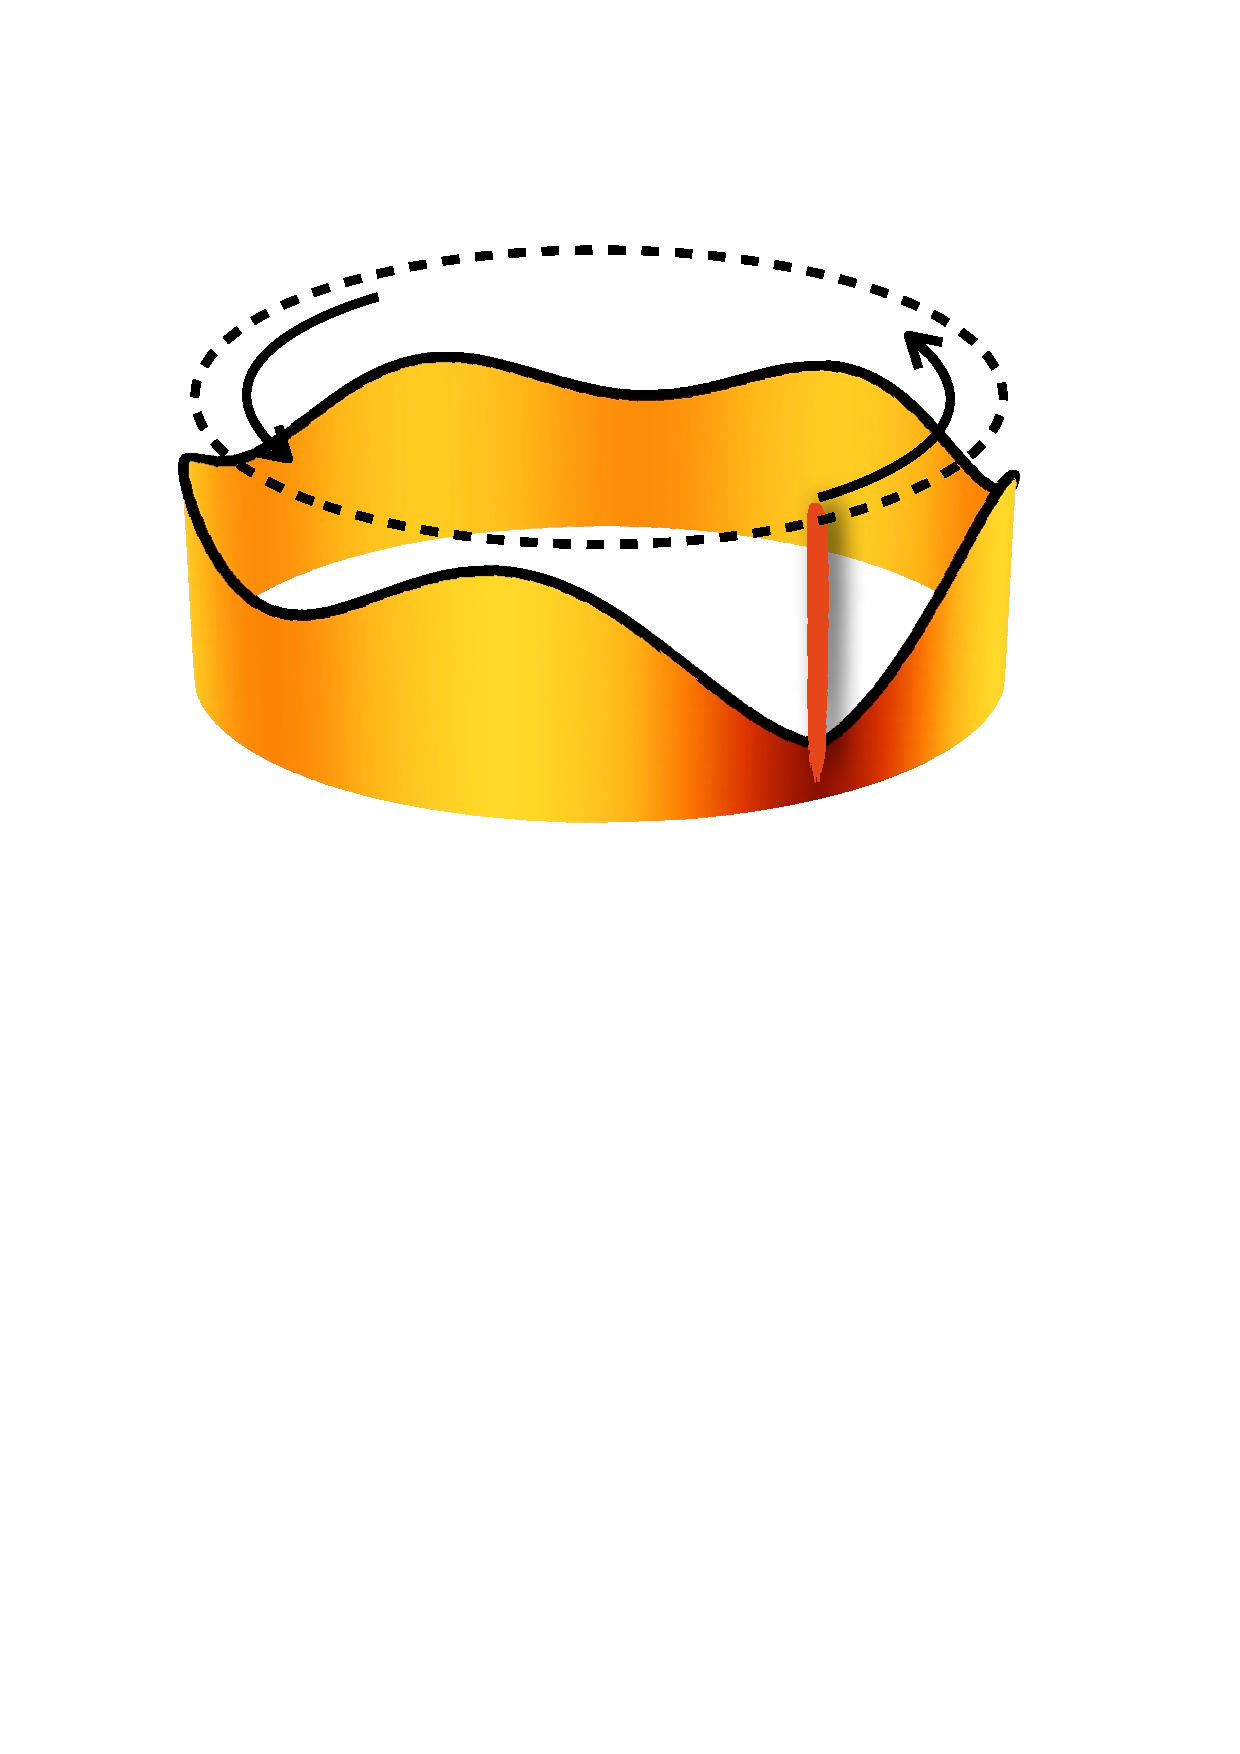
\includegraphics[width = 0.5\textwidth]{data/1d/scheme.pdf}
\caption{Schematic of the system.
Here, the density profile for five atoms in a TG gas is shown being stirred by a highly localized potential, indicated by the vertical line.}
\label{fig:ring_scheme}
\end{figure}

The energy spectrum of this system is shown in Figure~\ref{fig:avoid} as a function of the rotational frequency $\Omega \equiv \dot x_0 /L$ of the system.
In Figure~\ref{fig:avoid}(a) it is shown that in the absence of a barrier, when the eigenstates of $\mathcal{\hat H}$ are plane waves with quantized angular momentum in integer multiples of $2 \pi$, each angular momentum manifold exists separately such that the energy levels cross; however when $b>0$ (Figure~\ref{fig:avoid}(b)), the rotational symmetry is broken and avoided crossings appear in the energy spectrum.
This makes transitions between different manifolds possible~\cite{schenke2012}.

\begin{figure}

 \centering
 \subfigure{
 \centering
 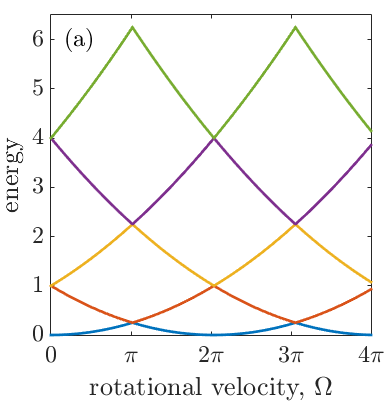
\includegraphics[width = 0.4\linewidth]{data/1d/cross.png}} 
 \subfigure{
 \centering
 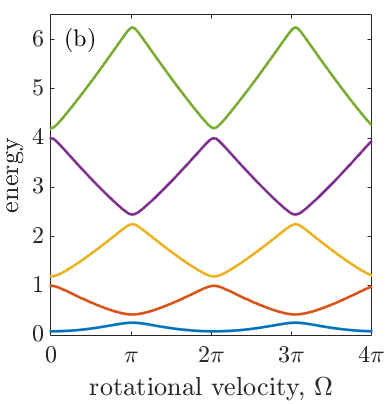
\includegraphics[width = 0.4\linewidth]{data/1d/nocross.png}}

\caption{Single-particle energy spectrum as a function of $\Omega$ for a barrier height of (a) $b = 0$ and (b) $b=2$.
When a barrier is present in the system, avoided crossings appear in the energy spectrum which grow as the barrier strength increases.}
\label{fig:avoid}
\end{figure}

By adiabatically accelerating the barrier's rotational frequency from 0 to $\pi$, a particle will enter a superposition between two rotational states, and in the case of the TG gas, this will create a macroscopic NOON superposition state between successive values of angular momentum~\cite{hallwood2010}.
This means that the manifolds will have an angular momentum of 0, 1, 2, $\ldots$, $N$, where $N$ is the number of particles in the system.
Any non-adiabatic behavior around the rotational frequencies of the avoided crossings can lead to a transition to a higher energy state and destroy the NOON state.
For this reason, the condition for adiabaticity must depend on the gap size, which is dictated by the barrier strength~\cite{nunnenkamp2008}; however, for a constant delta barrier, the gap size stays constant to first-order approximation~\cite{hallwood2007}.

Because this system requires adiabatic movement to properly generate the NOON state, it is difficult to efficiently generate it experimentally.
For this reason, it is a perfect example of a system where quantum optimal control and STA protocols can be used to rapidly engineer the appropriate states.
For quantum optimal control in this system, a non-adiabatic rotational frequency $\Omega(t)$ must be found, for which I will use the CRAB technique with an initial condition of $\Omega = 0$ and final condition of $\Omega = \pi$.
For each simulation in the fidelity landscape, this pulse will be modified with procedurally generated sinusoidal functions, the fidelity will be calculated, and then the Nelder--Mead method will be used to optimize the result.
This will allow one to determine an optimal pulse that maximizes the fidelity of the generated state when compared to the expected NOON state in a pre-set amount of time.
For this system, I will show the optimal pulse for the cases where I manipulate the rotational velocity, the barrier height, and both.

For STA protocols, the acceleration process will be split into two, one that breaks the rotational symmetry and another that accelerates the atoms.
At the end of the protocol, the potential is lowered to restore rotational symmetry.
Here, it is worth mentioning that a FAst, QUasi-ADiabatic (FAQUAD) shortcut for the creation of superposition states in a TG gas has also been created with some similarities~\cite{garaot2015}.

For both of these methods, instead of calculating the fidelity I calculate the \textit{infidelity}, which is simply $1-\mathcal{F} = 1-|\braket{\Psi|\Phi}|^2$, as the function to minimize.
It is also worth mentioning that the fidelity between two many-particle states in a TG gas can be calculated by using the method of mode projections~\cite{campo2011,lelas2011},
\begin{eqnarray}
\braket{\Psi | \Phi} &=& \frac1{N!} \sum_{\eta, \mu \in P} \epsilon_\eta \epsilon_\mu \braket{\psi_{\eta_1}(x_1) | \phi_{\mu_1}(x_1) } \cdots \braket{ \psi_{\eta_N}(x_N) | \phi_{\mu_N}(x_N) } \nonumber \\
\label{eq:fid}
&=&
\det \Big[ \braket{\psi_i | \phi_j }\Big]_{i,j=1}^N
\end{eqnarray}
which follows directly from the form of the TG state~\cite{girardeau1960}
\begin{equation}
\Psi(x_1,x_2,\ldots, x_N)= \frac1{\sqrt{N!}} \prod_{i<j}\textnormal{sign}(x_i-x_j) \sum_{\eta \in P} \epsilon_\eta \psi_{\eta_1}(x_1)\cdots\psi_{\eta_N}(x_N).
\label{eq:TG}
\end{equation}
Here $P$ represents the set of all permutations of $N$ elements, $\epsilon_\eta$ represents the anti-symmetric tensor of the permutation $\eta$, and $\psi_i$ represent the orbitals.
Now I will discuss the findings with both optimal control and STA protocols.


\subsection{Optimal control protocols}

\begin{figure}
 \centering
 \subfigure{
 \centering
 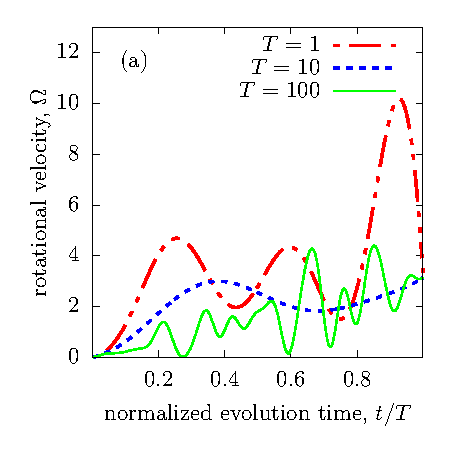
\includegraphics[width=0.45\textwidth]{data/1d/figR0.pdf}}
 \subfigure{
 \centering
 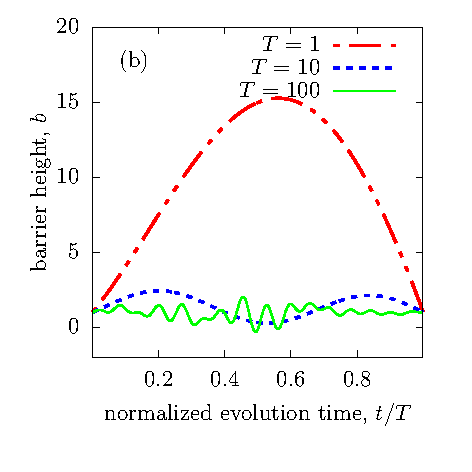
\includegraphics[width=0.45\textwidth]{data/1d/figB0.pdf}}
 \caption{Accelerating a single particle from the ground state with $J=15$.
 (a) Optimal rotational velocity pulses for $T = 1$, 10, and 100 for fixed barrier height $b=1$.
 (b) Optimal barrier height for a linearly increasing rotational velocity, $\Omega = \pi t/T$ for $T=1$, 10, and 100.}
 \label{fig:pulses}
\end{figure}

First, I will focus on the acceleration of a single particle, initially in the ground state of the system.
Figure~\ref{fig:pulses} (a) shows the results of this simulation if the barrier height is kept constant and one assumes an initial unmodified pulse that corresponds to a linear ramp from $\Omega = 0$ to $\pi$ for a preset total time, $T$.
For longer evolution times, there are many local maxima for the fidelity, and 
as such, longer evolution times effectively produce noisy signals and the Nelder--Mead method converges on one of many local minima.
For shorter evolution times, the pulse greatly affects the system and the shapes vary greatly from the initial linear ramp.
The infidelities for the linear guess pulse and its corresponding optimized pulse can be found in Figure~\ref{fig:lfid}, and one can see an improvement of several orders of magnitude.
Here, for longer evolution times, the initial linear pulse is a reasonable method to generate NOON states with an infidelity of $10^{-2}$ because it is already close to adiabatic; however, even in this case, the NOON state generation fidelity is better with optimization.
For all optimal control results in this chapter, the CRAB method was run 100 times and the data with the highest fidelity was kept.

For optimizations of the barrier strength, a simple linear ramp for $\Omega$ and an initial and final height for the barrier of $b = 1$ were chosen.
The optimal pulses for the barrier height for $T=1$, 10, and 100 are shown in Figure~\ref{fig:pulses}(b) and shorter evolution times similarly produce larger deviations from the initial pulse.
Again these pulses lead to significant improvements in the fidelity shown in Figure~\ref{fig:lfid}.

\begin{figure} 
\centering
 \subfigure{
 \centering
 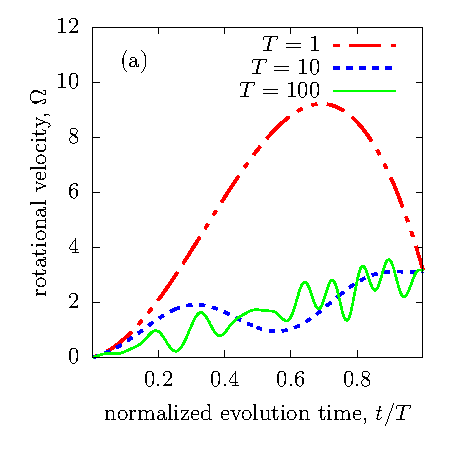
\includegraphics[width=0.45\textwidth]{data/1d/figR1.pdf}
 }
 \subfigure{
 \centering
 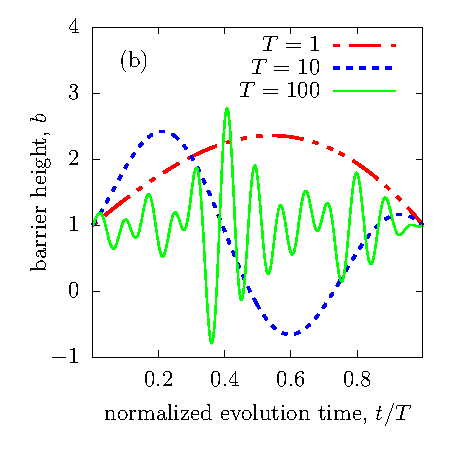
\includegraphics[width=0.45\textwidth]{data/1d/figB1.pdf}
 }
 \caption{
 Optimal pulses to accelerate a single particle initially in the ground state of the trap
 for $T = 1$, 10, and 100 for the (a) rotational velocity and (b) barrier height when optimizing over both simultaneously. }
 \label{fig:pulses_pair}
\end{figure}

With the CRAB method, it is possible to optimize over as many control parameters as one would like, and as such, it is possible to optimize over both the barrier strength and rotational frequency.
The results can be seen in Figure~\ref{fig:pulses_pair}, where (a) is the modified rotational frequency and (b) is the barrier height.
When comparing to the previous cases, similar trends emerge.
In particular, shorter evolution times result in less noisy optimizations when compared to longer evolution.
Even so, all sets of pulses are radically different when compared to optimizations over a single variable.
When comparing the fidelities in Figure~\ref{fig:lfid}, it is clear that optimizations over rotation alone provide the simplest method to optimize the fidelity.
It is likely that each run of the CRAB method is stuck in a local minimum in the fidelity landscape at some point and that optimization over both variables can provide the same optimization as rotating, alone.

\begin{figure}
 \centering 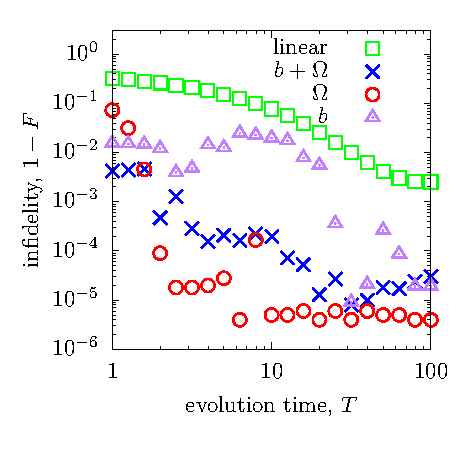
\includegraphics[width=0.5\textwidth]{data/1d/figlfid.pdf}
\caption{ Infidelities as a function of the overall process time for optimally controlled rotational acceleration, barrier height, or both.
Here, `linear' refers to an unoptimized linear acceleration from $\Omega = 0$ to $\pi$ while keeping the barrier height fixed at $b=1$.
}
\label{fig:lfid}
\end{figure}

\begin{figure}[t]
 \centering
 \subfigure{
 \centering
 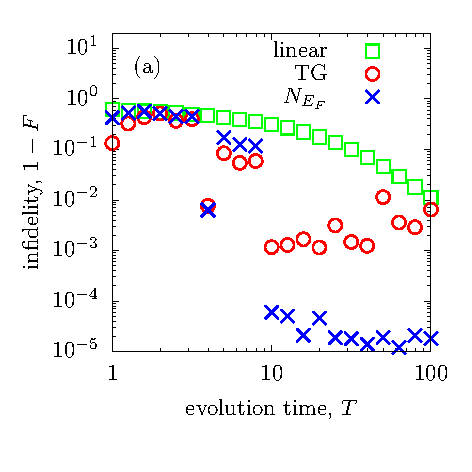
\includegraphics[width=0.45\textwidth]{data/1d/figTG3.pdf}
 }
 \subfigure{
 \centering
 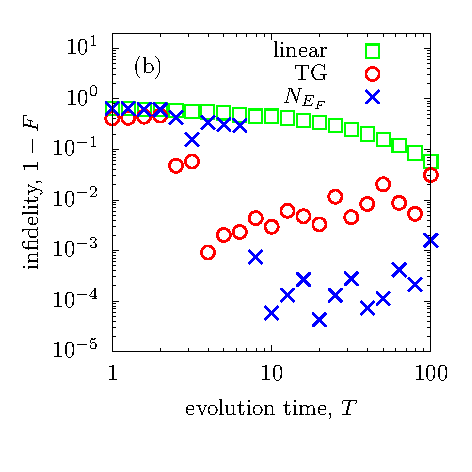
\includegraphics[width=0.45\textwidth]{data/1d/figTG5.pdf}
 }
 \caption{
Infidelities for the evolution of a TG gas with (a) $N=3$ and (b) $N=5$ particles using the CRAB optimal control technique.
The infidelities for optimized pulses with the particle at the Fermi edge is shown as blue crosses, and for the full TG gas as red circles.
Here, the green squares show the fidelity of a linear pulse for the atom closest to the Fermi edge.
A clear range where the CRAB algorithm is effective for generating NOON states with multiple particles can be clearly identified.}
 \label{fig:TGOC}
\end{figure} 


As such, when discussing the dynamics of a TG gas with 3 and 5 particles, I have only optimized over rotation.
Because of the Bose--Fermi mapping theorem, the evolution of an $N$-particle TG gas can be calculated by evolving a gas of $N$ spinless fermions.
In the zero-temperature limit, the fermions in the initial and target state create a Fermi sea by filling the lowest $N$ energy levels.
In this case, only atoms near the Fermi edge can transition into empty states and it is thus crucial to optimize the dynamics of the overall gas with respect to the particle with highest energy~\cite{garaot2015}.
In Figure~\ref{fig:TGOC}, I show the fidelity for the particle closest to the Fermi edge and the entire TG gas for $N=3$ and 5.
In this figure, one can see that by performing the optimization for the atoms near the Fermi edge, one can increase the fidelity of the entire gas for certain regimes; however, in contrast to Figure~\ref{fig:lfid}, there seems to be no fidelity increase from a linear pulse for short evolution times.
One can also observe what appears to be a crossover regime where optimizations of the particle at the Fermi edge seem to fail, but evolution of the entire gas is still slightly better than the linear pulse.
It is clear that the CRAB method creates highly effective pulses; however, for very short and long evolution times, the fidelity increase from a linear pulse is not as drastic.

\subsection{Results with STA protocols}

\begin{figure}
\centering
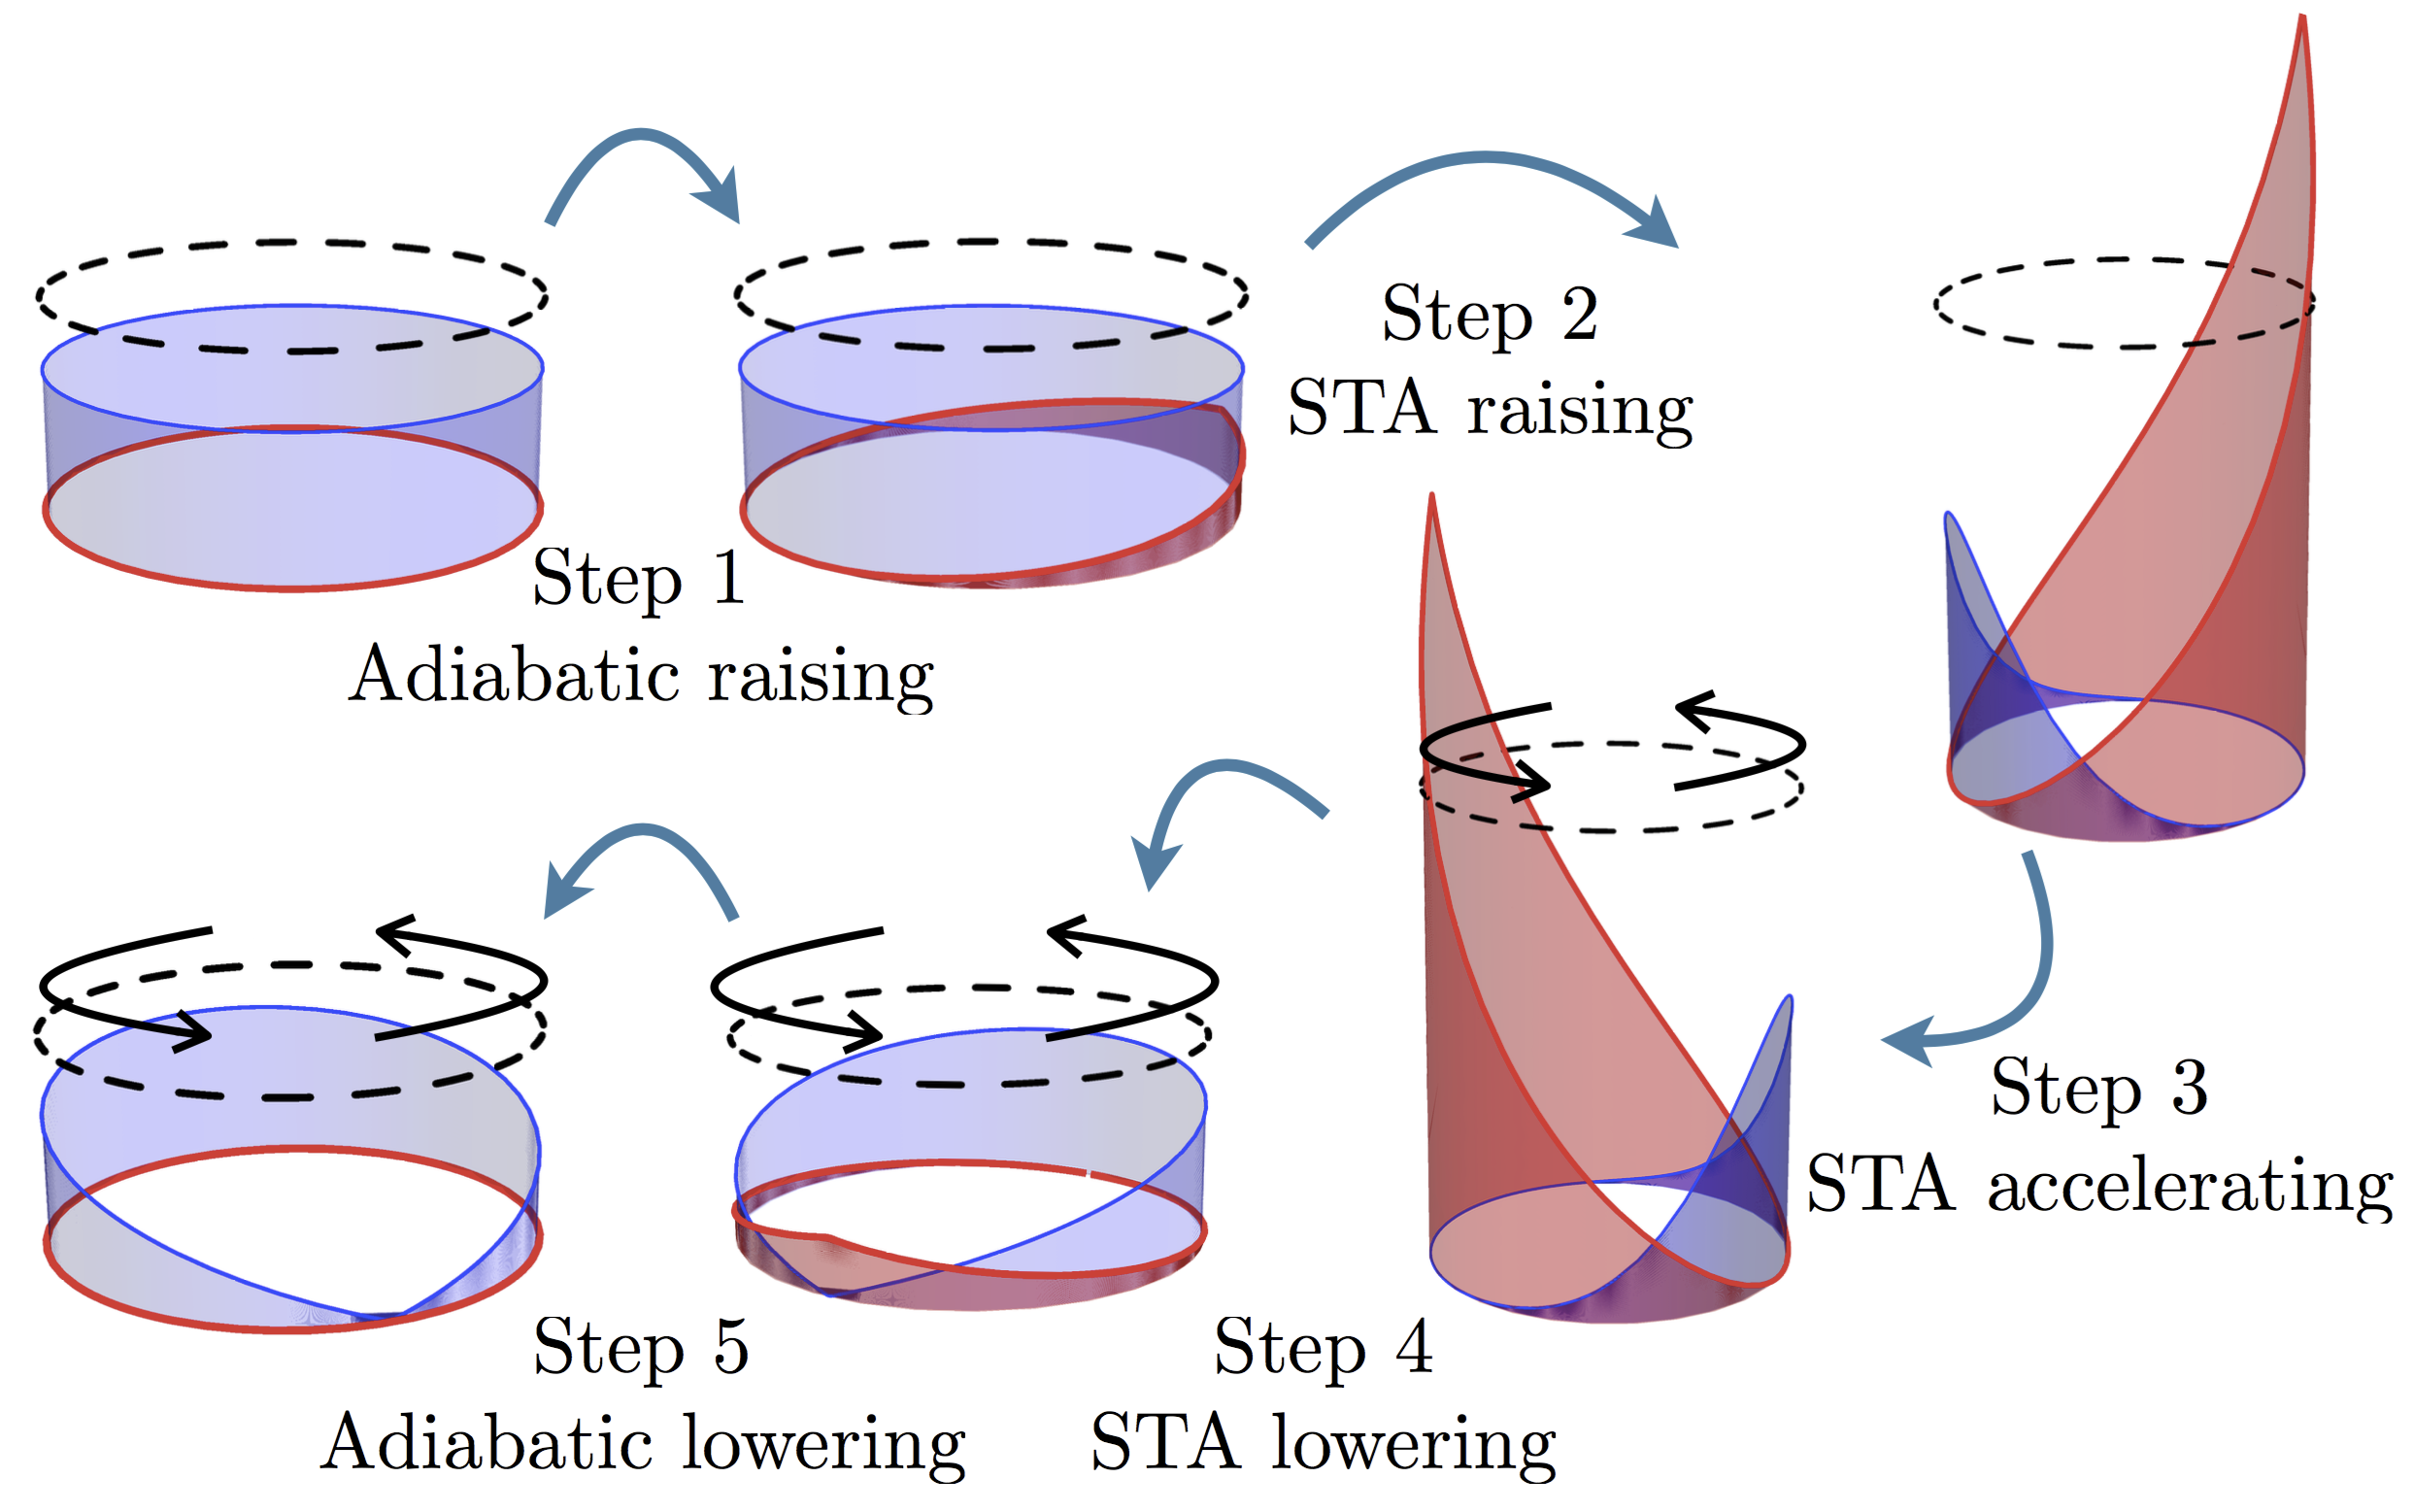
\includegraphics[width=0.8\textwidth]{data/1d/STAscheme.png} 
\caption{Scheme for the acceleration of a single atom using STA.
 In this example, the homogeneous ground state gets localized, accelerated and released at the angular velocity of $\Omega=\pi$ into the state
 $\left( \exp(i 2\pi x) +1 \right) /\sqrt 2$.
 The atomic density is indicated in blue and the potential is in red.}
\label{fig:STA-scheme}
\end{figure}


In this section, I will describe an STA protocol to generate NOON states in this system non-adiabatically, and though this was mentioned briefly in Section~\ref{sec:controltro}, it will be described more rigorously here.
In this case, I will start with rotational symmetry and break break this symmetry by introducing a time-dependent external potential at $t=0$ and removing it in the end.
For this, we do not choose a $\delta$ function, but instead a harmonic or sinusoidal potential along the ring.

The protocol consists of five steps:
\begin{enumerate}
\item Adiabatic raising of a weak harmonic or sinusoidal potential around the ring.
\item Fast tightening of this potential to localize the particles.
\item Accelerating the particles by moving the center of the potential.
\item Loosening the potential by reversing step 2.
\item Adiabatic lowering of the harmonic or sinusoidal potential.
\end{enumerate}
A schematic of this process is shown in Figure~\ref{fig:STA-scheme}.
For steps 2-4, pre-existing STA protocols can be used, and these will be discussed in this section.
The full protocol for the TG ring example will follow the STA methods outlined above with Lewis--Riesenfeld invariants and in this case, one needs to fulfill boundary conditions such that $\mathcal{\hat H}(t_0) = \mathcal{\hat H}(T)=p^2/2m$.
To be clear, the NOON states created with the STA protocol are slightly different those generated with quantum optimal control, as the STA variant does not rely on a $\delta$ barrier.

One of the two shortcuts explored for this system involves raising and lowering a harmonic potential~\cite{chen2010,chen20102}.
For this shortcut, a stationary harmonic potential is required and $F$, $x_c$, and $U$ from Equation~\eqref{eqn:HSTA} can all be set to zero, leading to
\begin{equation}
 \mathcal{\hat H}= -\frac{1}{2} \frac{\partial^2}{\partial x}+ \frac 1 2 \omega^2(t) x^2.
\end{equation}
\noindent To change the frequency while keeping the commutation relations and $\omega(t)$ continuous, one must impose the following conditions:
\begin{equation}
 \begin{array}{lcl}
\rho(t_0)=1, && \rho(t_f)=\gamma=\sqrt{\omega_0 / \omega_f},\\
\dot \rho(t_0)=0, && \dot \rho(t_f) =0, \\
\ddot \rho(t_0)=0, && \ddot \rho(t_f)=0.
\end{array} \label{eqn:squeeze}
\end{equation}

\noindent \noindent Which, together with Equations~\eqref{eqn:rho} and \eqref{eqn:squeeze} allow one to choose any form of $\rho$.
A good choice is the polynomial,
\begin{equation}
 \rho (s) = 6 \left(\gamma -1\right) s^5 -15 \left(\gamma-1\right) s^4 +10 \left(\gamma-1\right)s^3 + 1, \label{eq:rho_pol}
\end{equation}
\noindent where $s=(t-t_0)/(t_f-t_0)$ allows one to numerically find a solution for $\omega(t)$ that leads to the squeezing or expansion of the particle wavefunction with high fidelity in a short time.
As an important note, for small values of $\omega_0$, Equation~\eqref{eqn:rho} leads to purely imaginary values for $\omega(t)$, corresponding to repulsive potentials.
In order to avoid this and because the final states of this protocol require the external potential to be absent, the first and final steps in the protocol for this system involve adiabatically raising and lowering a potential to a suitable $\omega_0$ value. 

Once the potential has been raised, the particles are then accelerated to the chosen frequency, and a shortcut for this process with a harmonic trap exists~\cite{masuda2009,torrontegui2011,masuda2012}.
In the rotational shortcut, the trapping frequency is held constant and the position of the potential is modified.
This means that $U=0$, $F=\omega_0^2 x_0(t)$, and
\begin{equation}
 H= -\frac{1}{2} \frac{\partial^2}{\partial x}+ \frac 1 2 \omega^2_0 (x-x_0(t))^2.
\end{equation}
\noindent Here, Equation~\eqref{eqn:xc} becomes the only relevant auxiliary equation,
\begin{equation}
 \ddot{x}_c+\omega^2_0 (x_c-x_0)=0,
\end{equation}
and the conditions that must be imposed on $x_c$, are such that
\begin{equation}
 \begin{array}{lcl}
x_c(t_0)=x_0(t_0), && x_c(t_f)=d,\\
\dot x_c(t_0)=0, && \dot x_c(t_f) =\Omega_f, \\
\ddot x_c(t_0)=0, && \ddot x_c(t_f)=0,
\end{array}
\end{equation}
\noindent where $d$ is the final position of the potential minimum and $\Omega_f$ is its final velocity. 
For most applications of this shortcut, $d$ is important, and $\Omega_f$ is set to zero; however, this case is the opposite.

Like for the shortcut for raising the potential, the exact form of $x_c$ can be chosen somewhat arbitrarily, and a convenient choice is
\begin{equation}
 x_c(s)= (6 d -3 \Omega_f )s^5 - (15 d-7 \Omega_f )s^4+(10d-4 \Omega_f) s^3 + x_0(t_0),
\end{equation}
where, as above, $s$ is the normalized time.
The value of $\Omega_f$ can then be chosen to be odd multiples of $\pi$ to generate the desired NOON states based on the energy spectrum shown in Figure~\ref{fig:avoid}.

Unlike the shortcut to raise the potential, this shortcut is only approximate and works best when $\omega$ is large so that the particles are highly localized.
Both of these shortcuts rely on the presence of a harmonic potential of the form
\begin{equation}
 V_{H}(x,t)=\frac 1 2 \omega^2(t) \left( x-x_0(t)\right)^2, 
\end{equation}
where  $\omega$ is the frequency of the trap (in units of $\hbar/mL^2$) and $x_0$ the position of its minimum.
In the case of the TG ring, the potential must be symmetric around $x_0$, such that it is continuous at $x=\pm 1/2$; therefore, the real form of $(x-x_0)$ must be $(x-x_0+1/2)(\mathrm{mod~} 1)-1/2$.
The potential $V_H$ is then continuous everywhere on the ring, but its derivative is discontinuous at $x=x_0+1/2$ because this position is diametrically opposite to $x_0$.
Though $V_H$ is easy to work with theoretically, it is not necessarily experimentally realistic, and for this reason, we also consider a sinusoidal potential of the form~\cite{phelan2013,masuda2014},
\begin{equation}
 V_{S}(x,t)= \frac{\omega^2(t)}{2 \pi^2} \sin^2 \left(\pi \left( x-x_0(t)\right) \right) ,
\end{equation}
where the notation is the same as before. 
Here, prefactors are chosen such that $V_{H}$ is an approximation of $V_S$ around $x_0$.

\begin{figure}
\centering
\subfigure{
\centering
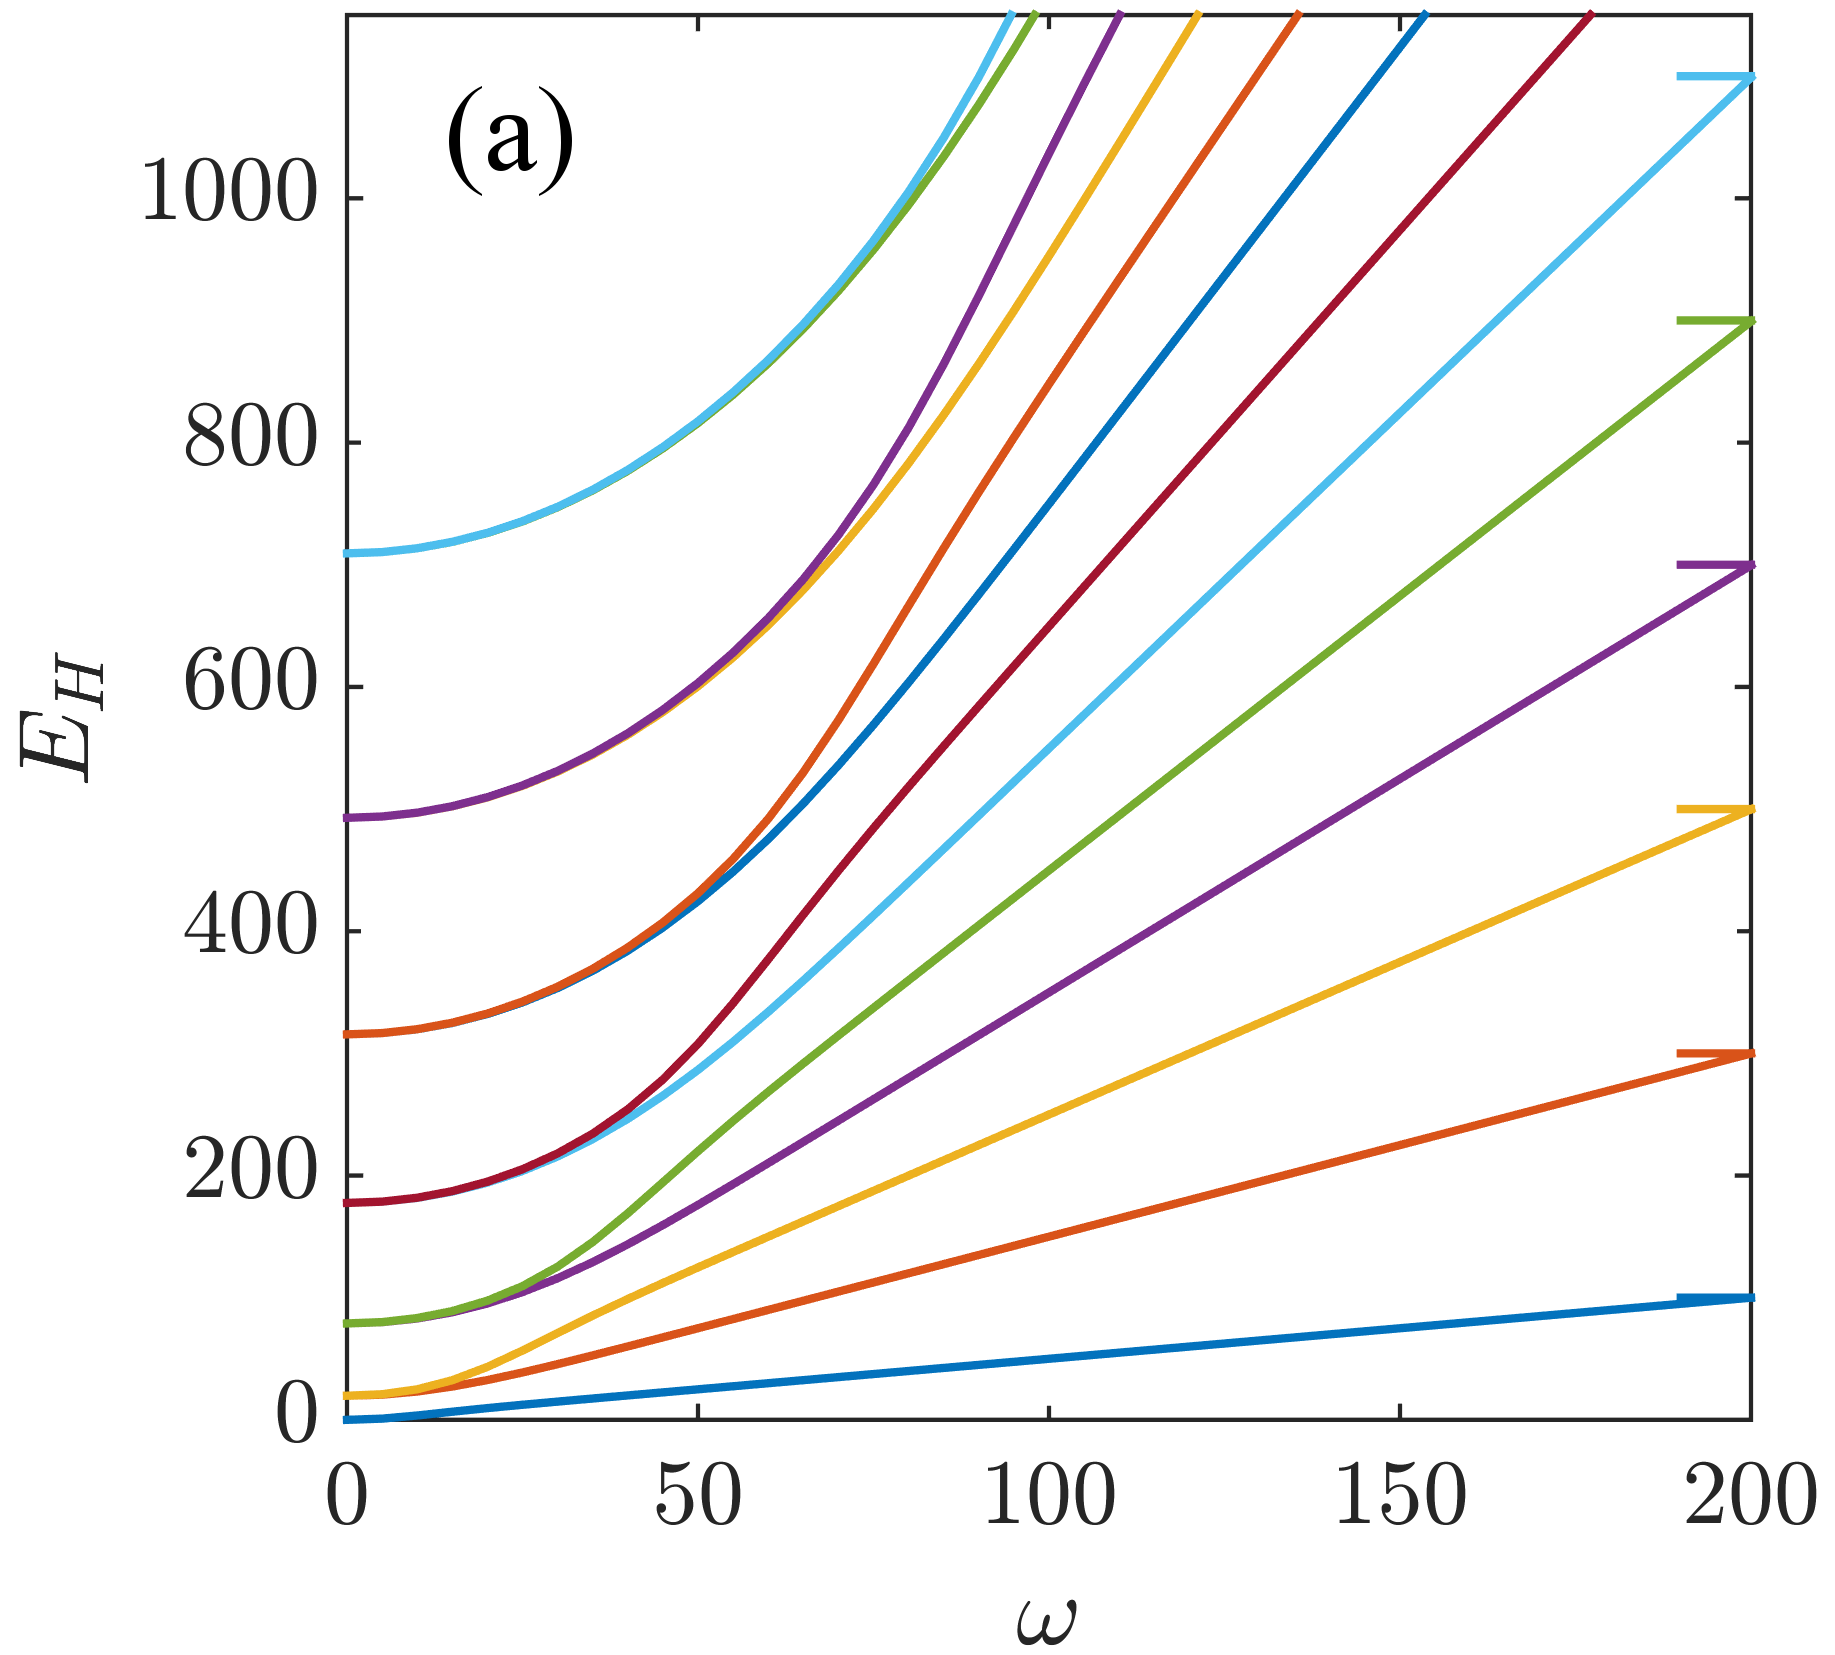
\includegraphics[width=0.48\linewidth]{data/1d/fig1.png}}
\subfigure{
\centering
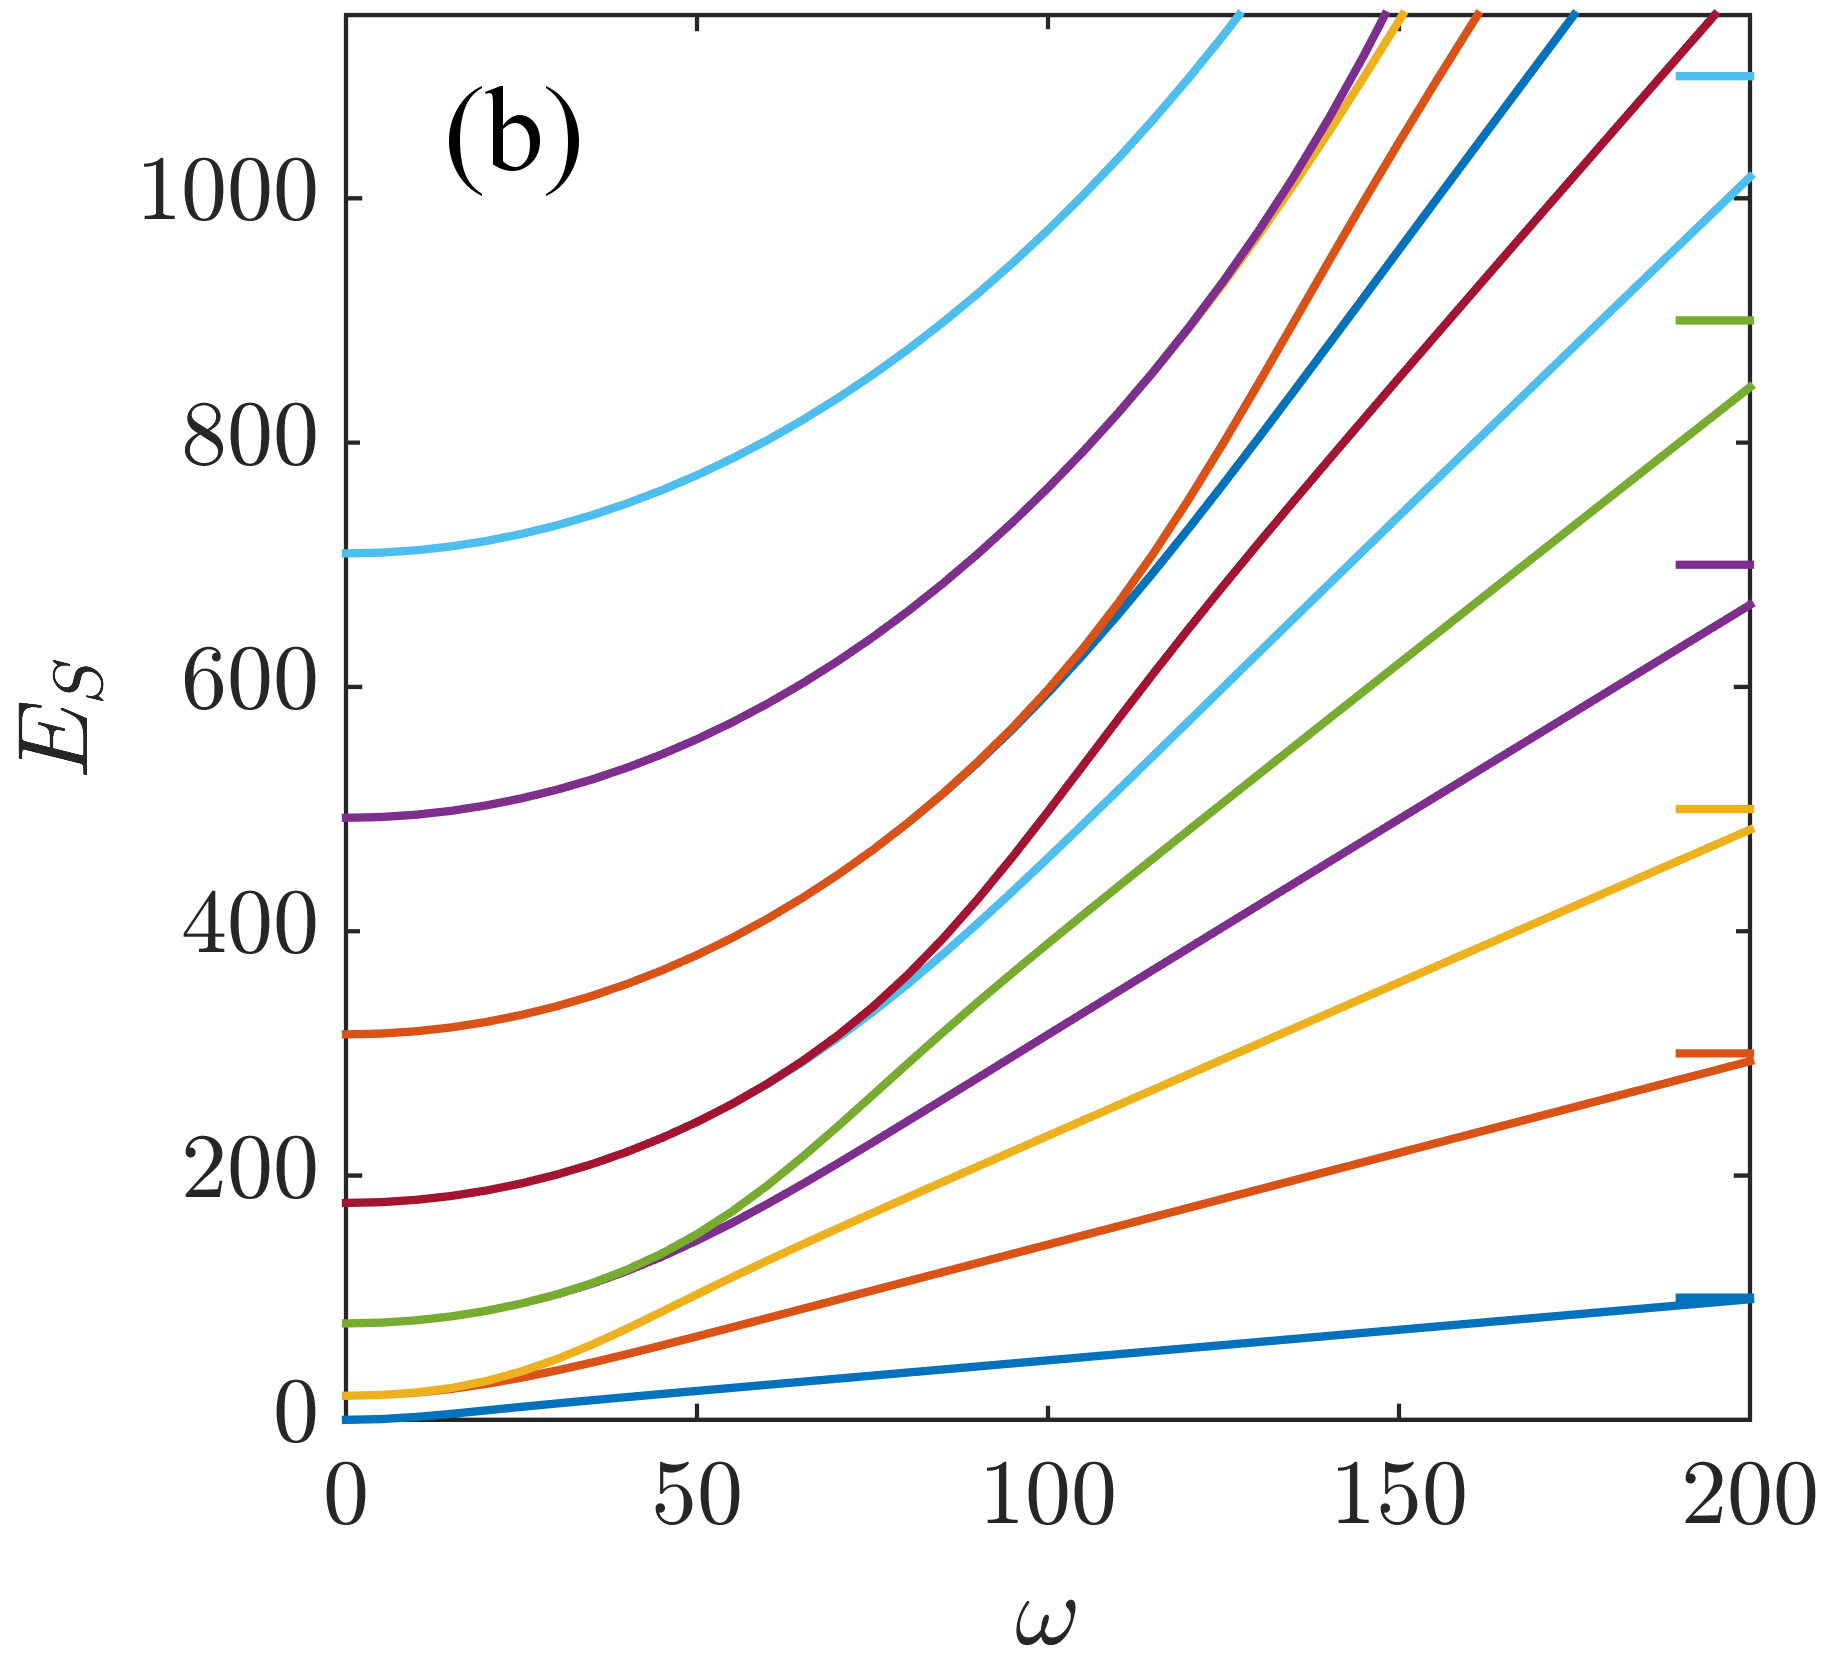
\includegraphics[width=0.48\linewidth]{data/1d/fig2.png}}

\caption{ Energy eigenspectrum of the system with (a) a harmonic or (b) a sinusoidal potential as a function of $\omega$. 
The eigenstates continuously change from angular momentum states of energy $E_k=2\pi^2 k^2$ (with $k=0,\pm1,\ldots$) at $\omega=0$, towards harmonic-oscillator states of energy $E_n=\omega(n+1/2)$ (with $n=0,1,\ldots$) for large $\omega$.
For comparison, the horizontal lines on the right vertical axis give the energy levels in a harmonic potential with $\omega=200$.}
\label{fig:spectrum}
\end{figure}

In Figure~\ref{fig:spectrum}, I show the difference between the two potentials by computing the energy spectra of both Hamiltonians.
Here, the eigenstates at $\omega=0$ are the angular momentum states $e^{i 2 \pi k x}$, with degenerate clockwise and counterclockwise momentum states of opposite quantum number $k$.
As $\omega$ is increased, the degeneracy ceases and the spectrum asymptotically approaches that of a harmonic oscillator.
For the sinusoidal case, the difference with the harmonic spectrum increases with the quantum number $n$.

\begin{figure}
\centering
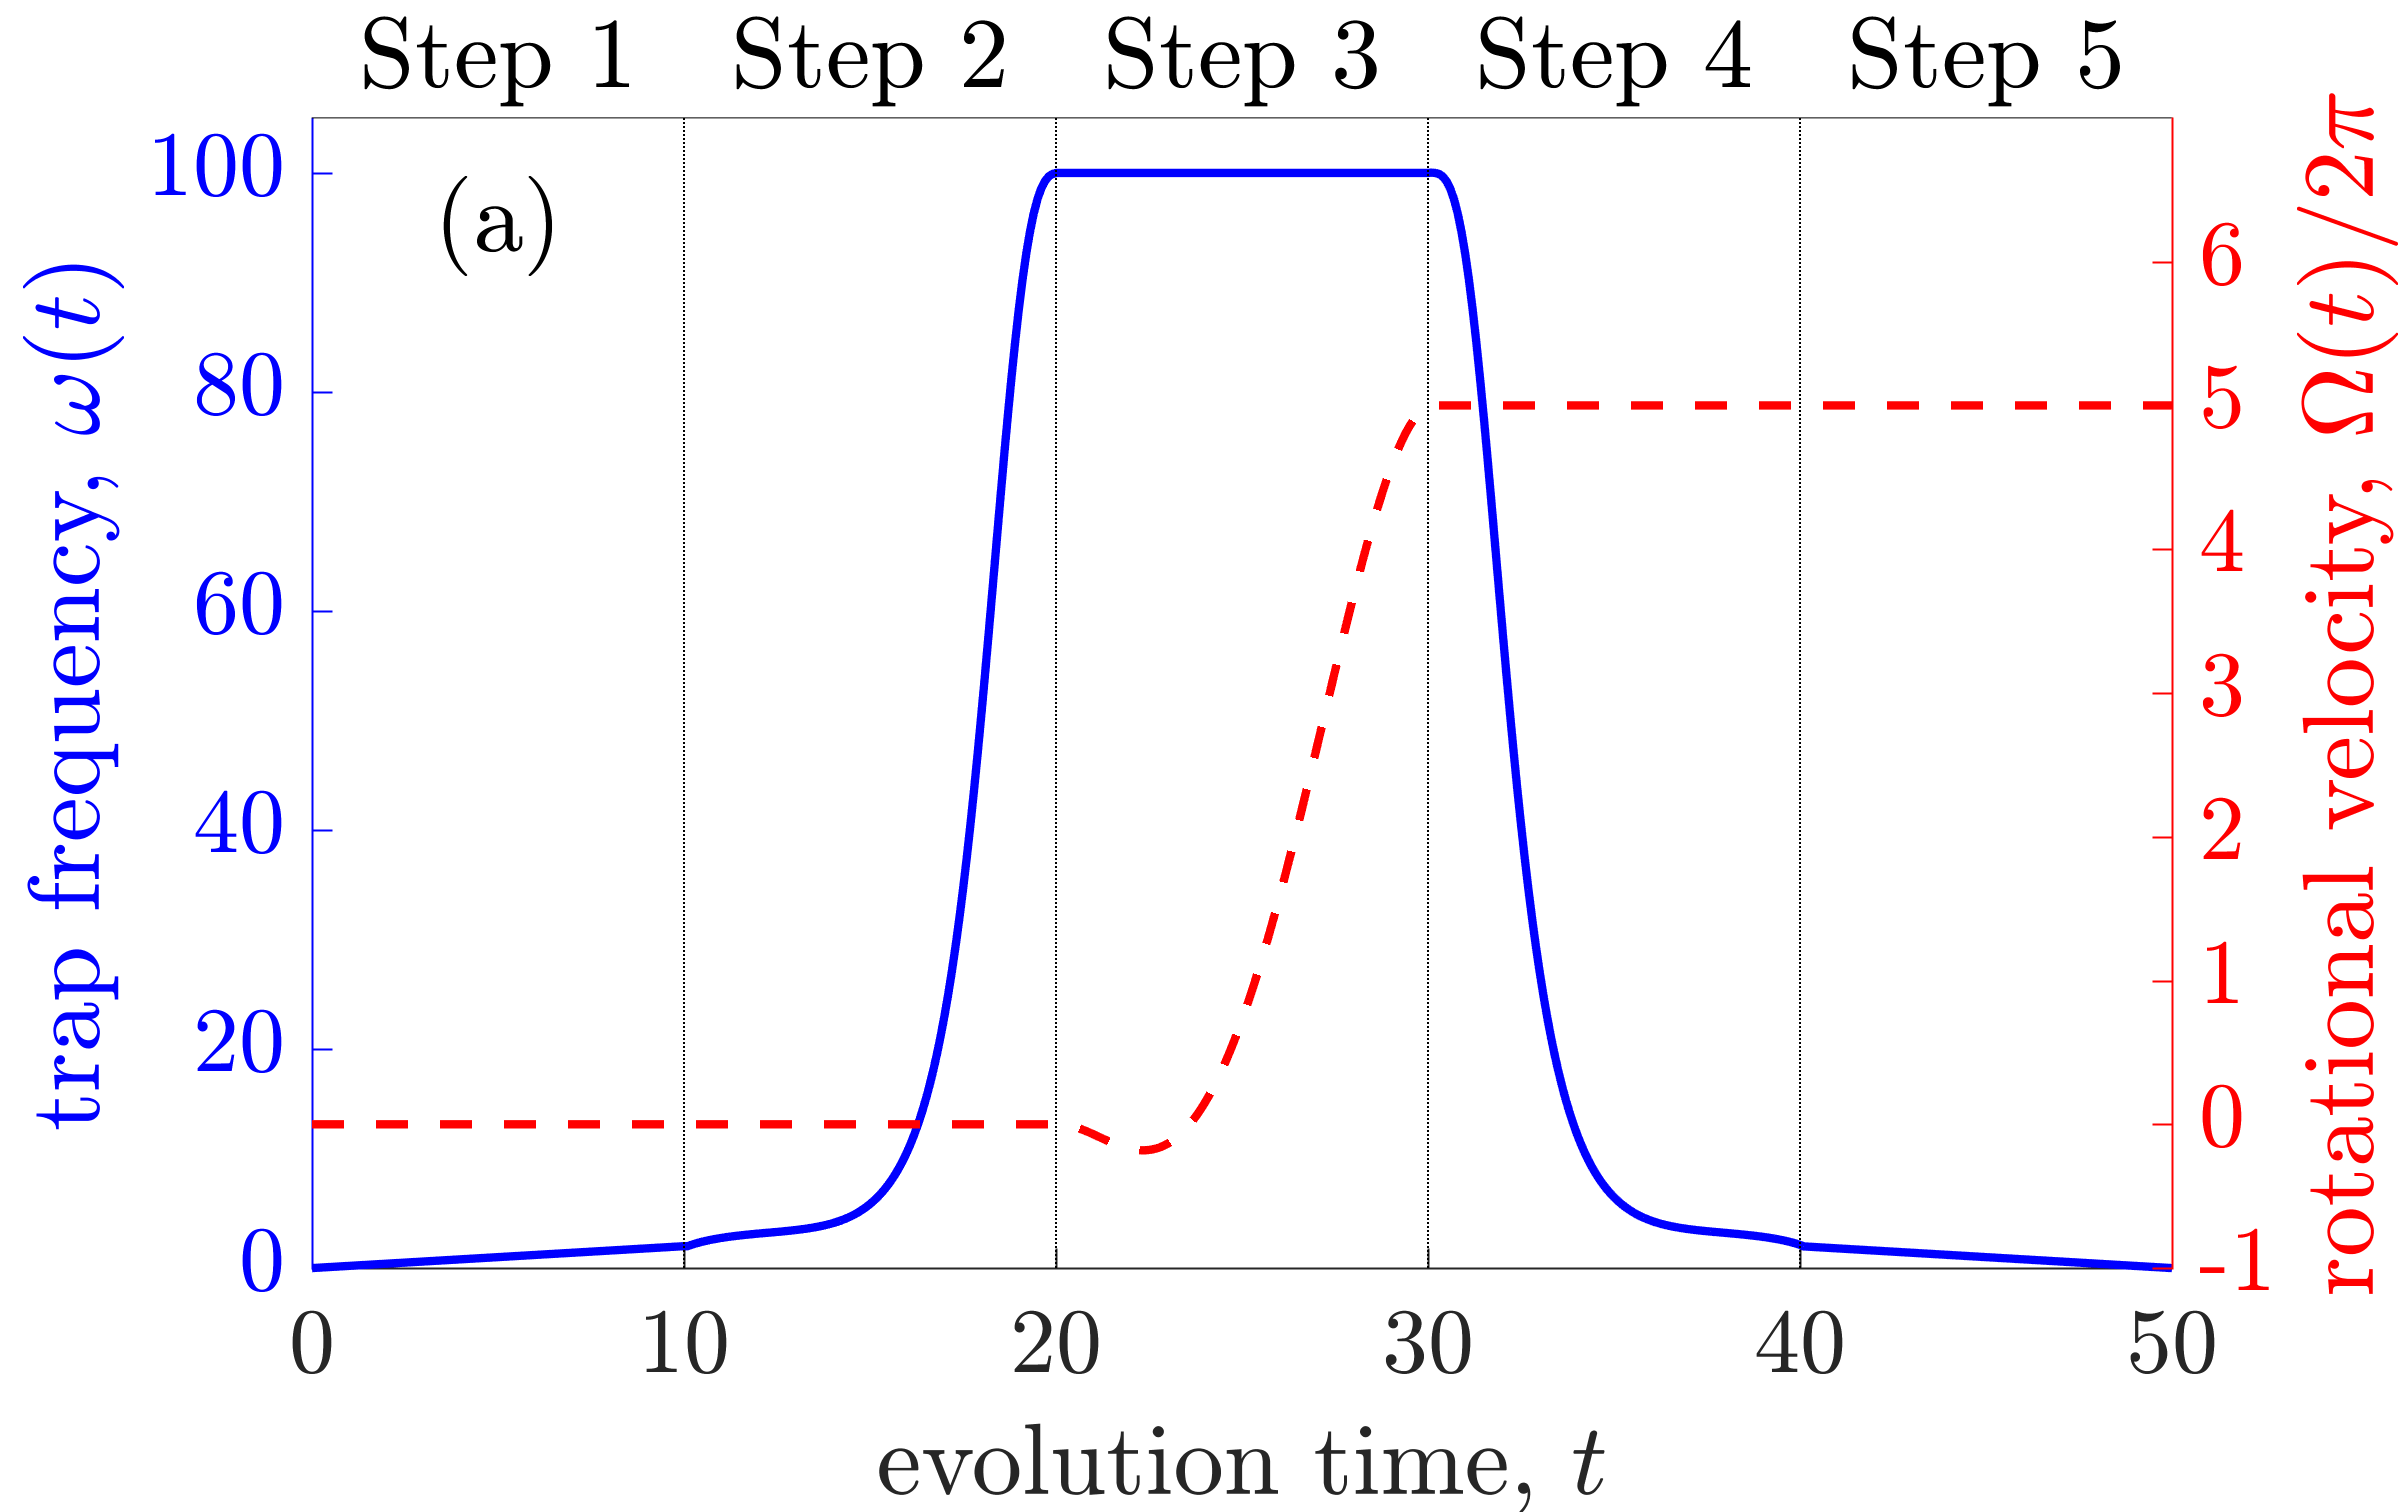
\includegraphics[width=0.45\linewidth]{data/1d/fig5.png}
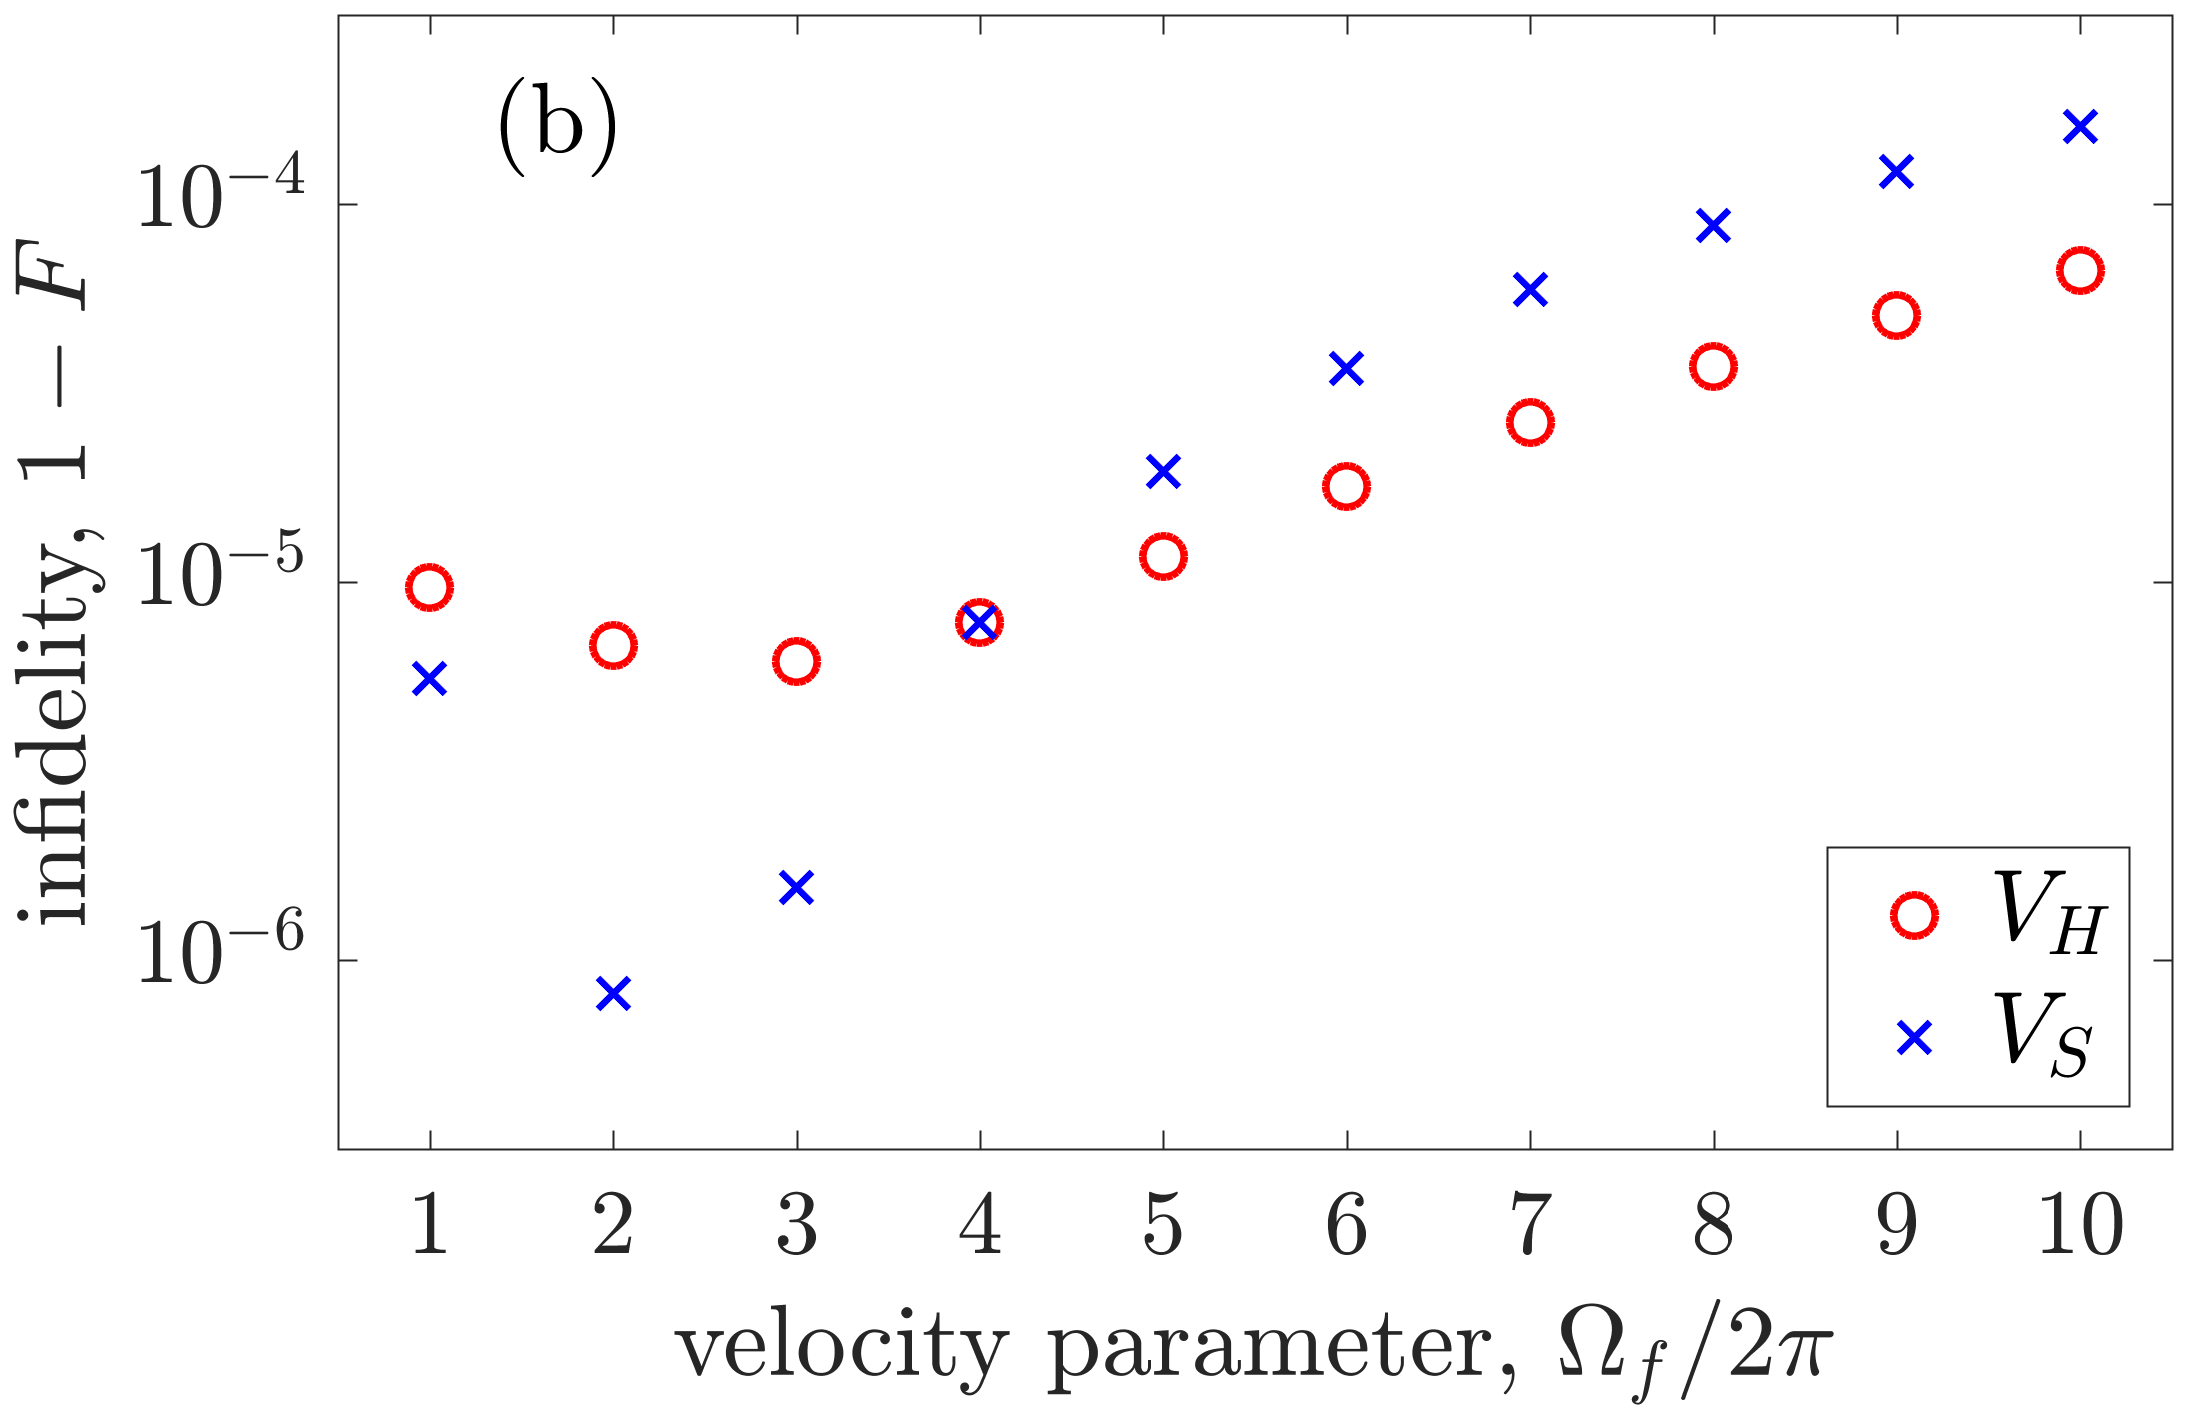
\includegraphics[width= 0.45\linewidth]{data/1d/fig6.png}
\caption{
(a) Plot of the parameters $\omega(t)$ and the angular velocity $\Omega(t)$ for the entire protocol.
The parameters are $\omega_0=2$, $\omega_f=100$, $d=100$, each step is executed in $t_f-t_0=10$, and $\Omega_f$ is picked depending on the desired output state (here, $\Omega_f=5 \times 2\pi$).
(b) Final infidelities for $\Omega_f=1,2,\ldots,10 \times 2\pi$ for $V_H$ (dotted blue line) and $V_S$ (solid red line).
The rest of parameters are as shown in (a).
}
\label{fig:final+param}
\end{figure}

Like the case of quantum optimal control, I will first show the single-particle results.
In Figure~\ref{fig:final+param}(a), the values for $\omega(t)$ and $\Omega(t)$ are shown, and
in Figure~\ref{fig:final+param}(b), the infidelities for the state preparation of plane waves $e^{i \Omega_f x}$ with $\Omega_f=1\ldots10 \times 2 \pi$ are shown.
Here, it is clear that even for a large amount of angular momentum, the fidelities remain high for both the harmonic and sinusoidal potentials.

For a multi-particle case in the TG regime, the initial states for the particles will be eigenstates of free space, which are simply plane waves $e^{i 2 \pi k x}$ with integer $k$.
Because the states with $\pm k$ are degenerate, it is equally valid to consider the initial eigenstates
\begin{align}
\phi^i_0(x)&=1,\\
\phi^i_{2l-1}(x)&=\frac{1}{\sqrt 2} \left( e^{i 2 \pi l x}-e^{-i 2 \pi l x} \right)= i \sqrt{2} \sin(2 l \pi x), \\
\phi^i_{2l}(x)&= \frac{1}{\sqrt 2}\left( e^{i 2 \pi l x}+e^{-i 2 \pi l x} \right) = \sqrt{2} \cos(2 l \pi x),
\end{align}
for $l=\{1,2,\ldots\}$.
These states have a total angular momentum of zero and are well-suited for the provided STA protocol because when an odd number of particles occupies the lower eigenstates, the sine and cosine pairs are guaranteed to be populated.

For $\Omega_f=\pi$, the plane wave of quantum numbers $k+1$ and $-k$ are degenerate and one can construct the target states
\begin{align}
\phi^t_{2l}(x)&=\frac{1}{\sqrt 2} \left( e^{i 2 \pi (l+1) x} + e^{-i 2 \pi l x} \right) = \sqrt{2} \cos[(2l+1) \pi x] e^{i \pi x} , \\
\phi^t_{2l+1}(x)&=\frac{1}{\sqrt 2} \left( e^{i 2 \pi (l+1) x}-e^{-i 2 \pi l x} \right) = i \sqrt{2} \sin[(2l+1) \pi x]e^{i \pi x} ,
\end{align}
for $l=\{0,1,2,\ldots\}$.
The states with total angular momentum $\pi$ are similar to NOON states.

\begin{figure}
\centering
\subfigure{
\centering
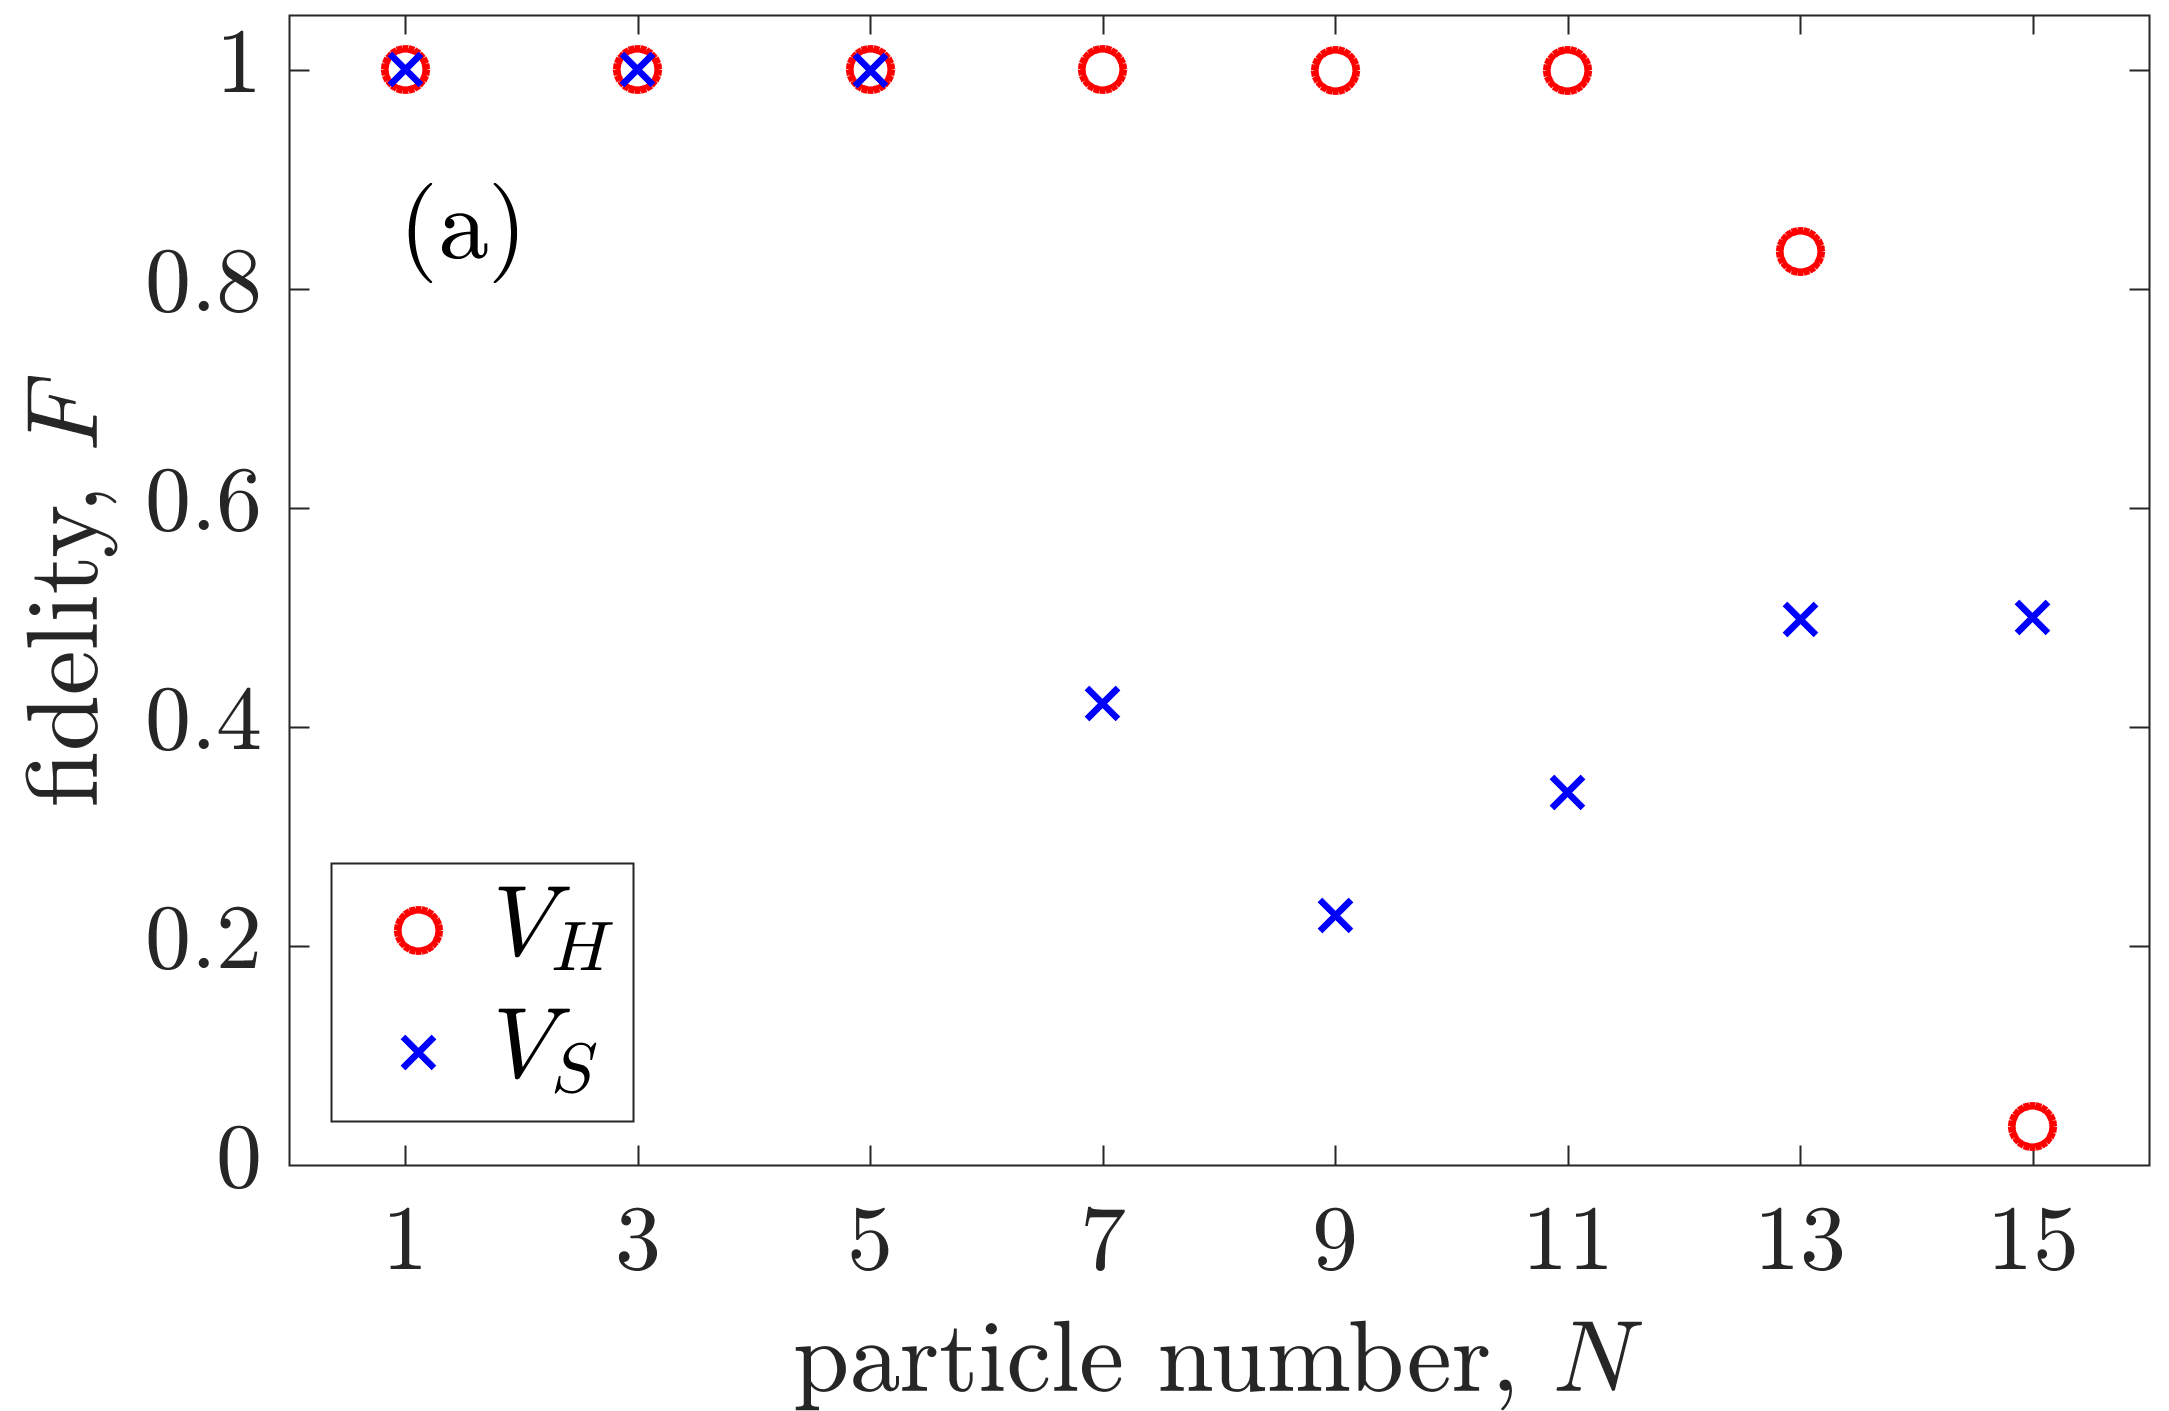
\includegraphics[width= 0.45\linewidth]{data/1d/fig7a.png} }
\subfigure{
\centering
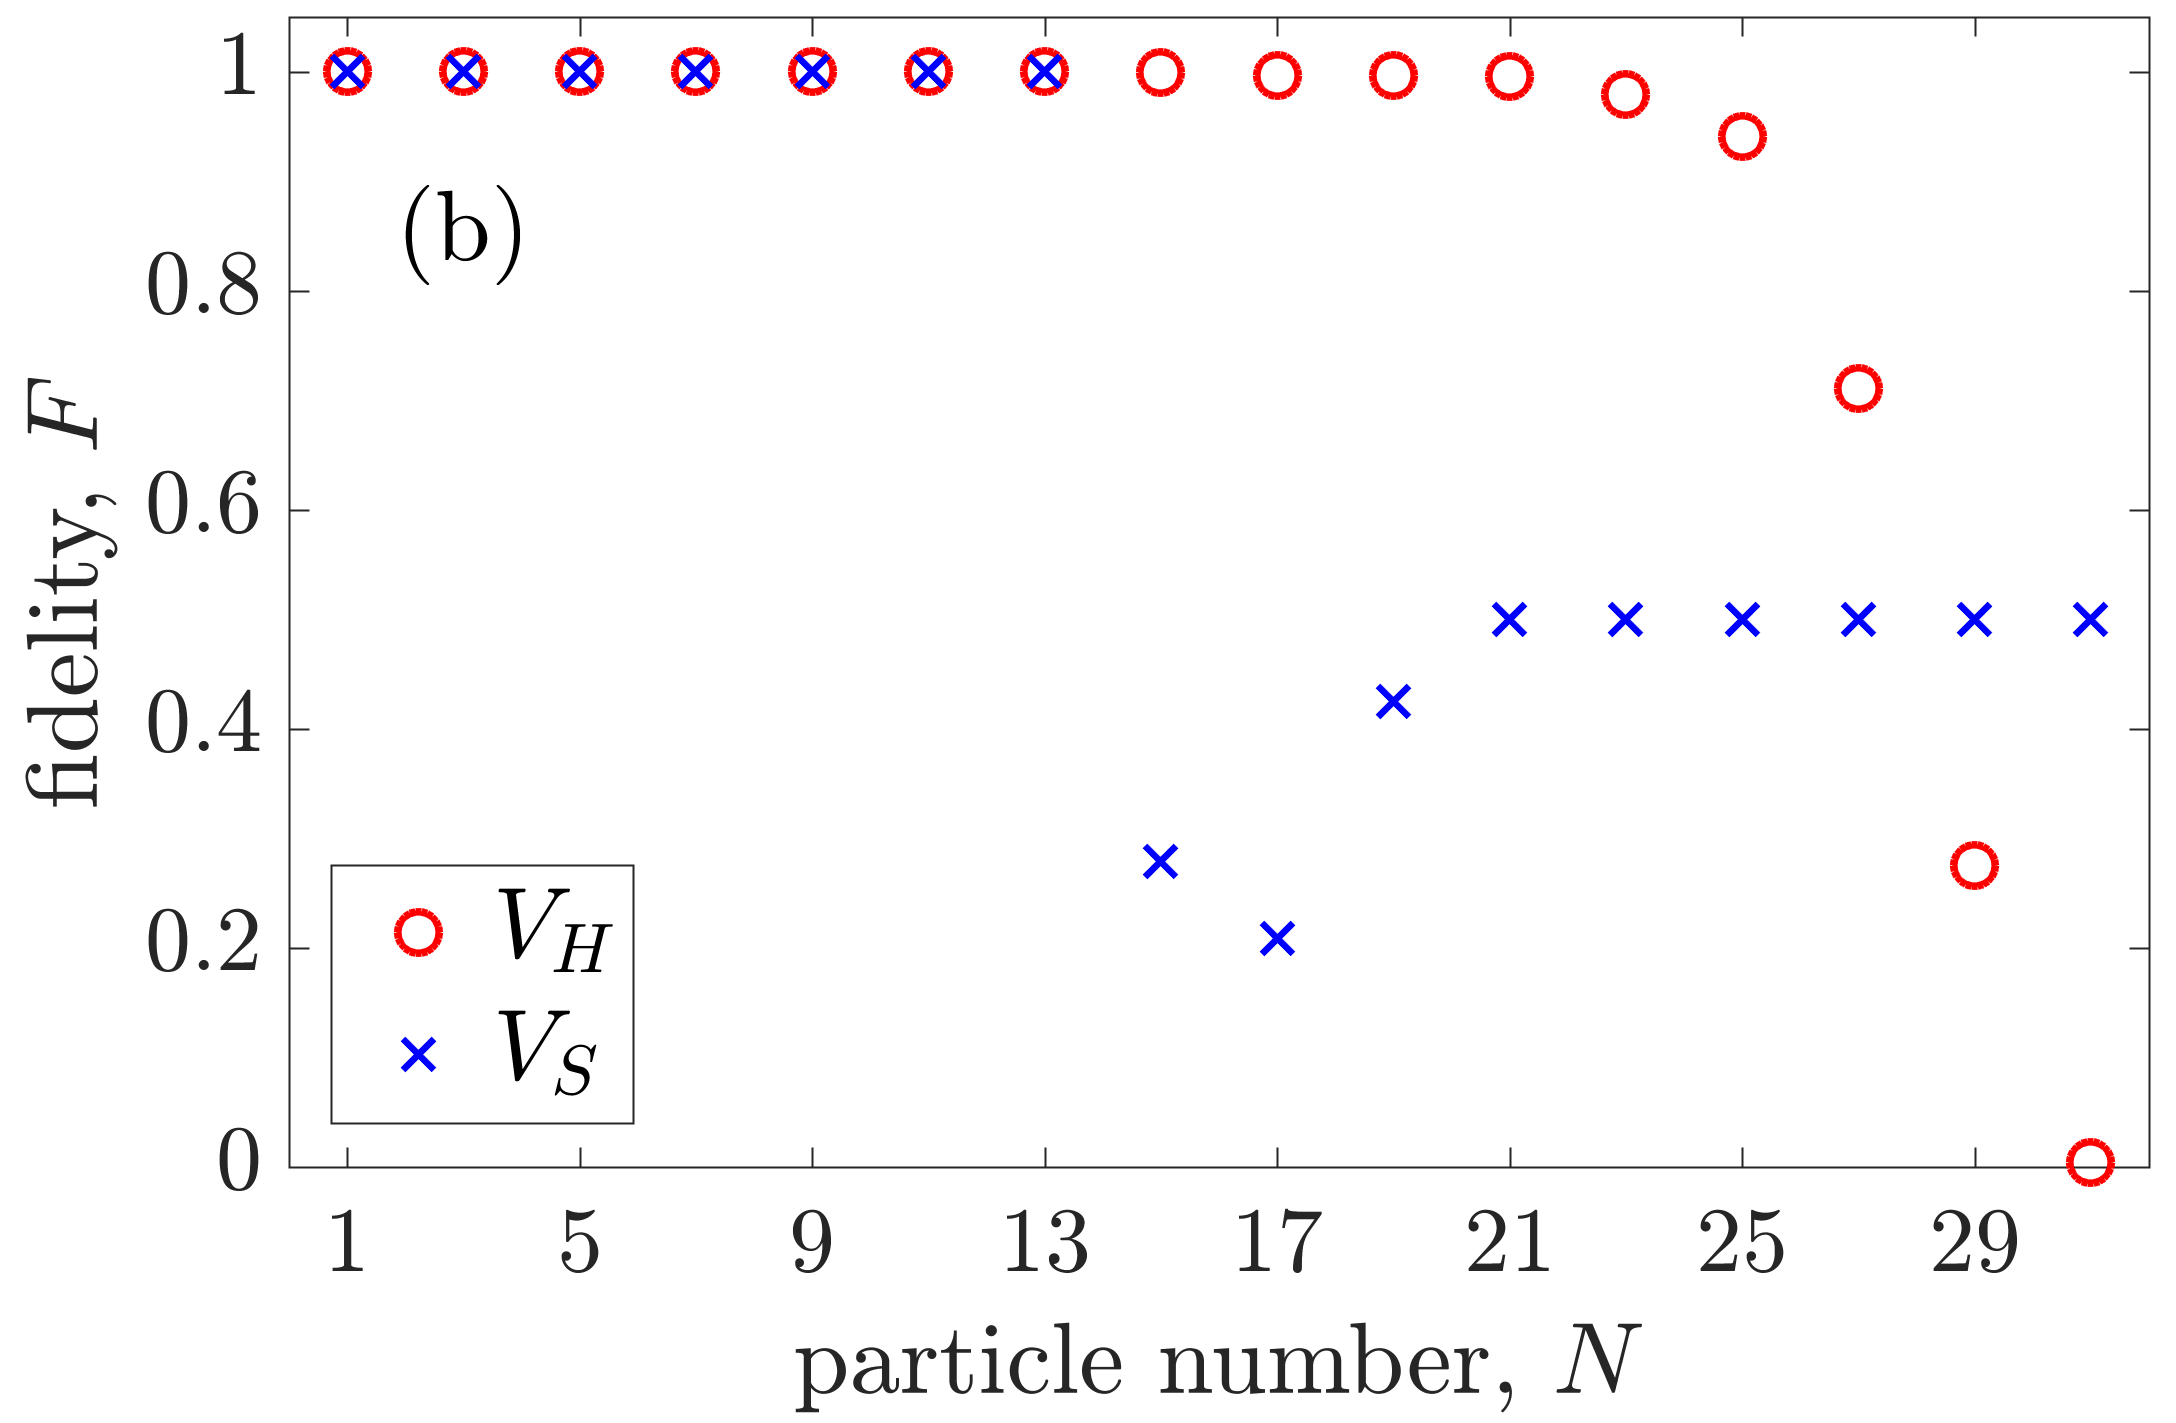
\includegraphics[width= 0.45\linewidth]{data/1d/fig7b.png}}
\caption{ Final fidelities $F$ of TG states of increasing particle number for the protocol shown in Figure \ref{fig:final+param}(a) with $\Omega_f = \pi$ for $V_H$ (red circle) and $V_S$ (blue cross). Plot (a) shows the fidelity of the protocol with $\omega_f = 100$ and (b) with $\omega_f = 200$.}
\label{fig:TG-STA}
\end{figure}

Any initial state $\ket{\phi^i_l}$ can be brought to the target state $\ket{\phi^t_l}$ with high fidelity with the proposed protocol, and the process also works for TG gases.
In Figure~\ref{fig:TG-STA}(a), the harmonic potential fidelities are shown to remain high for $N \leq 11$ after which they decrease due to a finite maximum height of the potential enforced by periodic boundary conditions.
The fidelities can be improved by increasing the maximum trapping frequency $\omega_f$ as was demonstrated in Figure \ref{fig:TG-STA}(b) where the value of $\omega_f$ is doubled and the fidelities remain high until $N \leq 21$.
When using the sinusoidal potential, the fidelity drops for smaller particle numbers compared to the  harmonic potential (although it also increases with $\omega_f$), due to the lower height $V_S$ has compared to $V_H$.

\section{Outlook}

In this chapter, quantum optimal control and STA protocols were introduced to optimize quantum engineering tasks in cold atomic gases.
I have introduced a physical system to generate NOON states in a TG gas non-adiabatically with both methods, and they were shown to be highly effective.
Such dynamical evolution techniques require time-dependent control parameters, such as rotation frequency or barrier height, and allowing for these dynamic operations has hitherto been a difficult task on GPU hardware.
In the following chapter, I will discuss GPU hardware in-depth and also tackle this issue, along with several others noted in Chapter~\ref{ch:splitop}.


\chapter{Vortex analysis of two-dimensional superfluid systems}
\label{ch:2d}

Here, we show an application of the GPUE codebase in simulating a two-dimensional chaotic system with few vortices.
This chapter makes heavy use of the vortex tracking, rotation, and phase-imprinting methods described in Chapter~\ref{ch:gpu}.
In addition, this chapter intends to display the dependence of post-processing metrics to dynamical studies of superfluid systems.

In a similar fashion to Chapter~\ref{ch:1d}, this chapter will start with a disclaimer about the dimensionality of the systems we will be simulating.
In principle, all real-world physics is three-dimensional, but in a similar fashion to how a one dimensional cigar-shaped BEC can be created, a pancake-like geometry can also be constructed by increasing the trapping frequency in the $\hat z$ (perpendicular) direction with respect to the $\hat x$ and $\hat y$ (transverse) directions.
With this geometry, we can assume that the condensate is in the ground state along the $\hat z$ dimension and rewrite the wavefunction as $\Psi(\mathbf{r},t) = \Psi(x, y, t)\phi(z)$, where $\Psi(x, y, t)$ is the wavefunction in the transverse plane and $\phi(z) = (m \omega_z/(\pi\hbar))\text{exp}(z^2 m\omega_z/(2\hbar))$ is the ground state along the $\hat z$ dimension.
By integrating over $\hat z$, we also find that the interaction strength is modified for a two-dimensional consensate to be

\begin{equation}
g_{2D} = g \sqrt{\frac{m\omega_z}{2\pi\hbar}}.
\end{equation}

\noindent With these changes, we can simulate two-dimensional quantum simulations with the GPUE codebase~\cite{zhang2019, o2017, o2016topo, o2016}.

This chapter will apply several of the techniques mentioned in Chapters~\ref{ch:splitop} and \ref{ch:gpu} to a rotating two-dimensional BEC system for a small number of vortices and will follow the work of Zhang \textit{et.al.}~\cite{zhang2019}.

\section{Chaotic few-body vortex dynamics in rotating Bose--Einstein condensates}

Chaotic evolution is typically identified by a significant divergence in trajectory based on a small change in the initial conditions~\cite{strogatz2018}, and it is possible to find such an environment in turbulent flows~\cite{spiegel1987, biferale2005}.
For classically turbulent flow, the degree of chaos depends on the Reynolds number~\cite{berera2018}; however, the nature of quantum turbulent effects is still an active area of research~\cite{white2014}.
Because superfluid vortices are relatively simple compared to their classical counterparts, there has also been significant interest in the differences between classical and quantum turbulence~\cite{nemirovskii1995,kyriakopoulos2014,koukouloyannis2014,navarro2013}.
In spite of the differences between the fluid models, vortex dynamics in superfluid systems are remarkably similar to classical point-vortex models and key features of classical turbulence, such as the Kolmogorov spectrum have been shown to exist for large, turbulent, quantum systems~\cite{nore1997,stalp1999,araki2002,salort2010}.

In this study, we would like to create a quantum system that is chaotic without relying on quantum turbulence, and
it is known that it is not possible to excite quantum chaos in large vortex lattices, as these systems have been proven to be stable to external perturbations~\cite{o2017}.
For this reason, we wish to probe quantum chaos with a small number of vortices, such that quantum tuburlent effects are not excited.
These chaotic, few-vortex systems have been studied previously by Aref and Pomphrey~\cite{aref1982, aref1980, aref1983}, who showed that quantum chaos can be excited in systems with as few as four vortices in an infinite plane~\cite{aref1982}.
Unlike classical chaos, the onset of quantum chaos seems to appear with fewer vortices present, and few-vortex systems have been explored experimentally for two, three, and four vortices in harmonically trapped BECs~\cite{navarro2013}.
When analyzed with a reduced Hamiltonian approach, harmonically trapped BECs seem exhibit chaotic effects with as few as three vortices, two co-rotating vortices and an anti-vortex rotating in the other direction~\cite{kyriakopoulos2014,koukouloyannis2014}.

Experimentally, it is now possible to detect vortex circulation~\cite{seo2017}, image vortices in-situ~\cite{wilson2015}, and probe vortex dynamics at different times within a single experiment~\cite{freilich2010, serafini2017}.
Because quantum vortices are simple and BECs are highly controllable experimental systems in two-dimensions, there has been significant interest in two-dimensional quantum turbulent systems as well~\cite{neely2013,shin2004}.
Additional effects, such as the K\'arm\'an vortex street~\cite{kwon2014} and Onsager vortex clusters~\cite{gauthier2018,johnstone2018} have also been shown to exist experimentally.

In order to engineer well-controlled initial conditions, we will create a small vortex lattice of four vortices, and then create a small defect via phase imprinting.
This process will controllably induce chaotic vortex dynamics in an experimentally feasible way.
We also show that these chaotic dynamics are enhanced by the close approach of vortices in the simulated results.
By using phase imprinting in this way on a larger number of vortices in a vortex lattice, it might be possible to induce chaotic events there as well, which might enable studying a set of vortex trajectories that is chaotic at specific points, but stable overall.

\section{Model}

\begin{figure}
\center 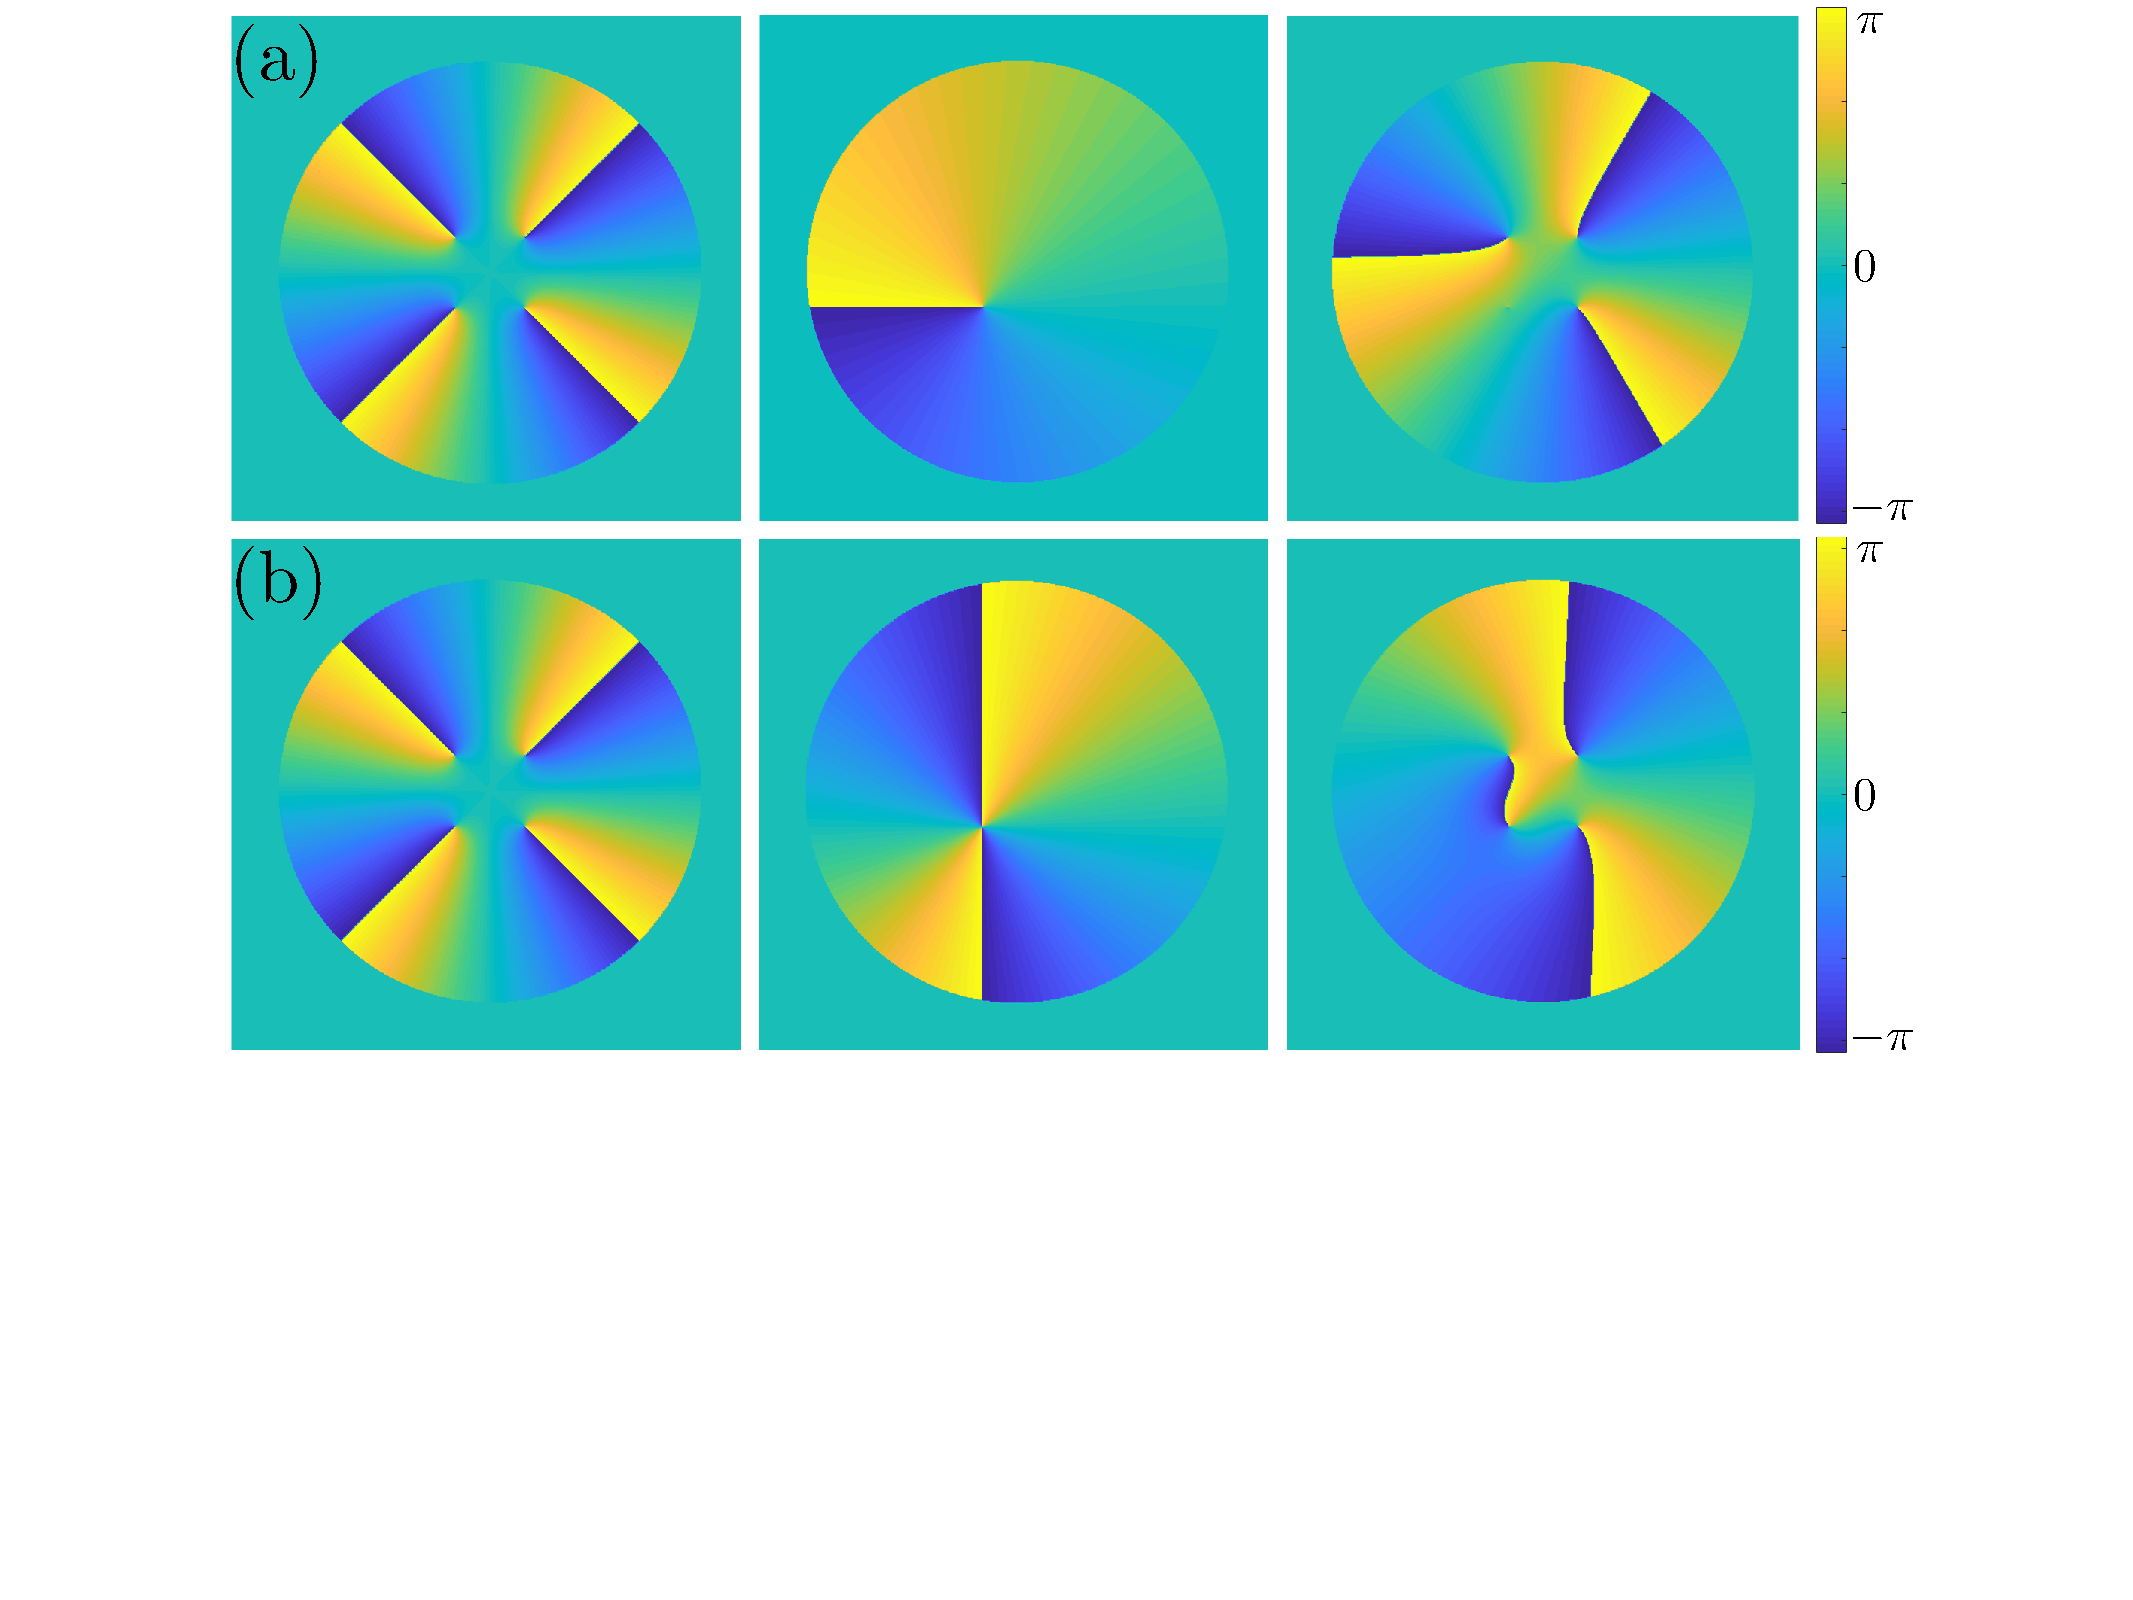
\includegraphics[width=0.75\textwidth]{data/2d/phase/phase}

\caption{
The initial four co-rotating vortex system is shown at the left.
In the center is the applied phase mask of $-2\pi$ for (a) and $-4\pi$ for (b), and the resulting phase distribution is shown on the right.
Here we see that by applying a $-2\pi$ phase winding, we erase a vortex from the system, and by applying a $-4\pi$ phase winding, we flip the vortex, creating an anti-vortex.
}
\label{fig:phase}
\end{figure}


For this study, we created a condensate with $N = 10^6$ $^{87}$Rb atoms with an s-wave scattering length of $a_s \approx 90a_0$ in a pancake geometry with typical trapping frequencies of $(\omega_\perp, \omega_z) = (2\pi, 32\pi)$Hz.
Here, the s-wave scattering length is $a_s \approx 90a_0$ and the effective interaction strength is $g = 6.8\times 10^{-40}$ m$^4$kg/s$^2$.
These simulations were performed on a grid of $2^{10} \times 2^{1-}$ points and covering an extent of $700\mu \text{m} \times 700 \mu \text{m}$

First, ground-state evolution was performed with a low rotation frequency of $\Omega = 0.3 \times 2\pi$ Hz via GPUE~\cite{schloss2018}.
Though large rotational frequencies will create a triangular lattice, for smaller frequencies, other configurations are known ~\cite{aftalion2001}, and we will focus on the regine where the ground state is composed of four vortices in a square configuration~\cite{zampetaki2013}.
Once this configuration is achieved, we then manipulate a vortex via phase imprinting, such that three co-rotating vortices and one anti-vortex exist in the system.
Examples of phase imprinting on this system can be seen in figure~\ref{fig:phase}, where the top row shows a simple vortex annihilation and the bottom row shows a vortex flip.

\section{Regular and irregular vortex dynamics}

\begin{figure}
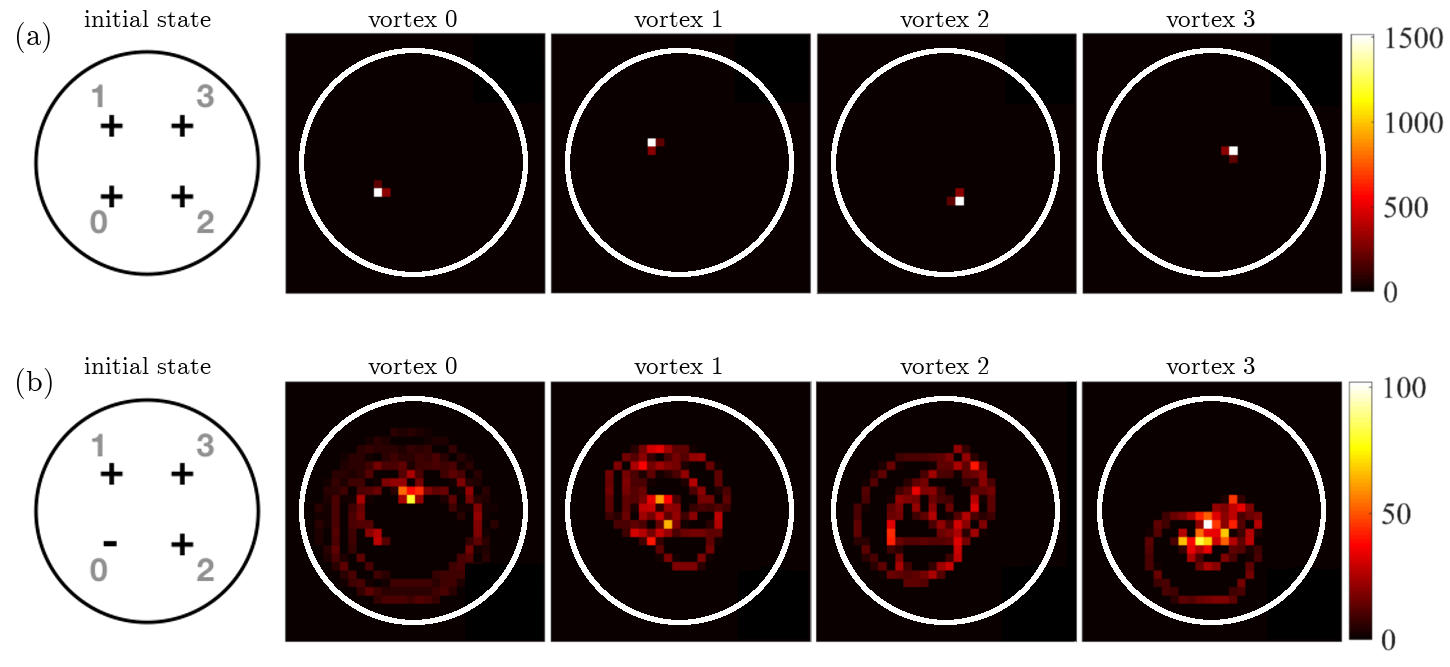
\includegraphics[width=\textwidth]{data/2d/histogram/histogram}

\caption{
Histograms of the positions of each vortex in the transversal plane for 20 secons in the co-rotating frame.
The lower left vortex has been annihilated and re-imprinted with (a) the same and (b) the opposite direction of rotation, exactly on the location of the previous vortex.
The area of each plot is $400\mu \text(m) \times 400 \mu \text{m}$, and the white circles correspond to iso-lines at 40\% the maximum density to highlight the extent of the vortex motion.
In (a), we see that if all four vortices are co-rotating, regular trajectories appear, but in (b), we see that flipping the rotation direction of a single vortex creates disordered trajectories.
}
\label{fig:histogram}
\end{figure}

It is known that a lattice of vortices with the same direction of rotation will exhibit regular dymanics~\cite{abo2001}, and in Figure~\ref{fig:histogram}(a), we confirm this for a system of four vortices.
In this figure, we show a histogram of the vortex trajectory over 20 seconds of evolution when removing and then re-imprinting a vortex of the same rotational direction at the same location
Even though a small residual movement appears due to small phonon excitations that were not fully removed from the imaginary time evolution, the vortices remain stationary.
In Figure~\ref{fig:histogram}(b), we also show that if the re-imprinted rotation is of the opposite direction, the vortex dynamics become more disordered, with vortices traversing a larger width of the condensate.
It is worth mentioning that these histograms can be constructed experimentally with available imaging techniques~\cite{wilson2015,freilich2010}.

\begin{figure}
\center 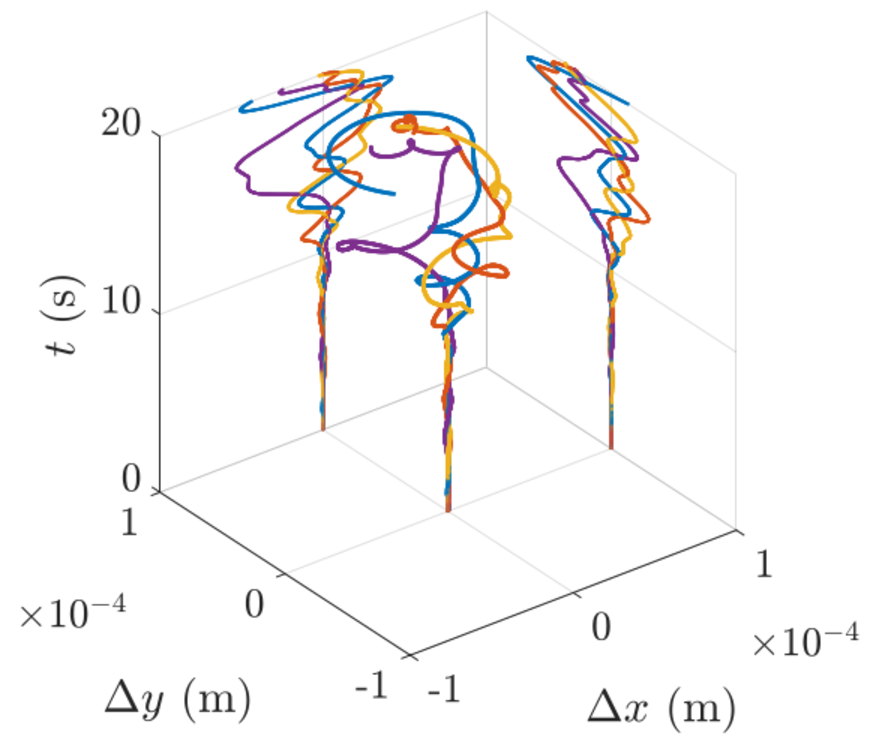
\includegraphics[width=0.5\textwidth]{data/2d/evolution/evolution}

\caption{
Evolution of the difference in trajectories $\triangle \textbf{r}_i = \textbf{r}_{i}-\textbf{r}'_{i}$ with $\textbf{r}$ corresponding to the position of the $i$th vortex from the center of the condensate and $i\in \{0,\ 1,\ 2,\ 3\}$ labelling each individual vortex for the four-vortex system as shown in Fig.~\ref{fig:histogram}.
A small change in the initial position of the anti-vortex arises from a phase-imprint at $(x_{0},y_{0})$ and $(x_{0}-\xi/3,y_{0})$ where $(x_{0},y_{0})$ denotes the pre-existing co-rotating vortex core position.
The curves show that even though the onset of disorder is immediate, a strong divergence of trajectories is observed at about $t\approx 10 \text{s}$ (see projections onto the $x$-$t$ and $y$-$t$ planes).
The difference in trajectory of the anti-vortex, $\Delta \mathbf{r}_0$, is shown in blue, while yellow, orange, and purple lines depict the three co-rotating vortices.
}
\label{fig:evolution}
\end{figure}

Even though the introduction of the anti-vortex creates a disordered trajectory, it could be entirely possible that this trajectory is stable.
To uniquely identify chaotic behaviour, we need to show that any small perterbation in the vortex location will also provide a significantly different trajectory.
To check this, we compare two sets of vortex trajectories with slightly different shifts in the initial position of the anti-vortex, $\mathbf{r}_0$ and $\mathbf{r}'_0$, where $\mathbf{r}_0 - \mathbf{r}'_0 = \xi/3$ and $\xi$ is the healing length.
In Figure~\ref{fig:evolution}, we show the differences in trajectories, defined as $\Delta \mathbf{r}_i(t) = \mathbf{r}_{i}(t)-\mathbf{r}'_{i}(t)$ in Figure.~\ref{fig:histogram}, where $\mathbf{r}$ refers to the position of the $i$th vortex from the center of the condensate and $i\in \{1,2,3\}$ corresponds to the vortex number.
Here, we see that the difference in trajectory is initially small, but diverges significantly at around $t \approx 10$ seconds, which is a strong indication of chaotic behavior.

After closely inspecting the vortex dynamics (shown in the supplementary movie~\ref{movie}), we see that this strong divergence in vortex trajectories seems to be accelerated when all four vortices come in close proximity.
Because the velocity fields of each vortex decays as $1/\mathbf{r}$, where $\mathbf{r}$ is the distance from the core, the vortices experience stronger velocity fields when they are closer; therefore, the point of minimal separation can be seen as a highly nonlinear multi-vortex scattering event that accelerates the divergence shown in Figure~\ref{fig:evolution}.
In Figure~\ref{fig:snapshots} we study this further by showing snapshots of the condensate density before ($t = 6$s), at ($t = 10$s), and after ($t = 15$s) the scattering event are shown in (a) and (b) for the non-shifted and shifted anti-vortex locations.
The differences between position of each vortex and the anti-vortex is also shown (b) for the case where the anti-vortex is shifted by $\xi/3$.
Here, we see that there is a clear minimum at $t \approx 10$s, which is the same time at which the  trajetories begin to diverge in Figure~\ref{fig:evolution}
In order to characterize this divergence in trajectory, we must analyze the vortex dynamics in more detail and calculate the Lyapunov exponent

\begin{figure}
\center 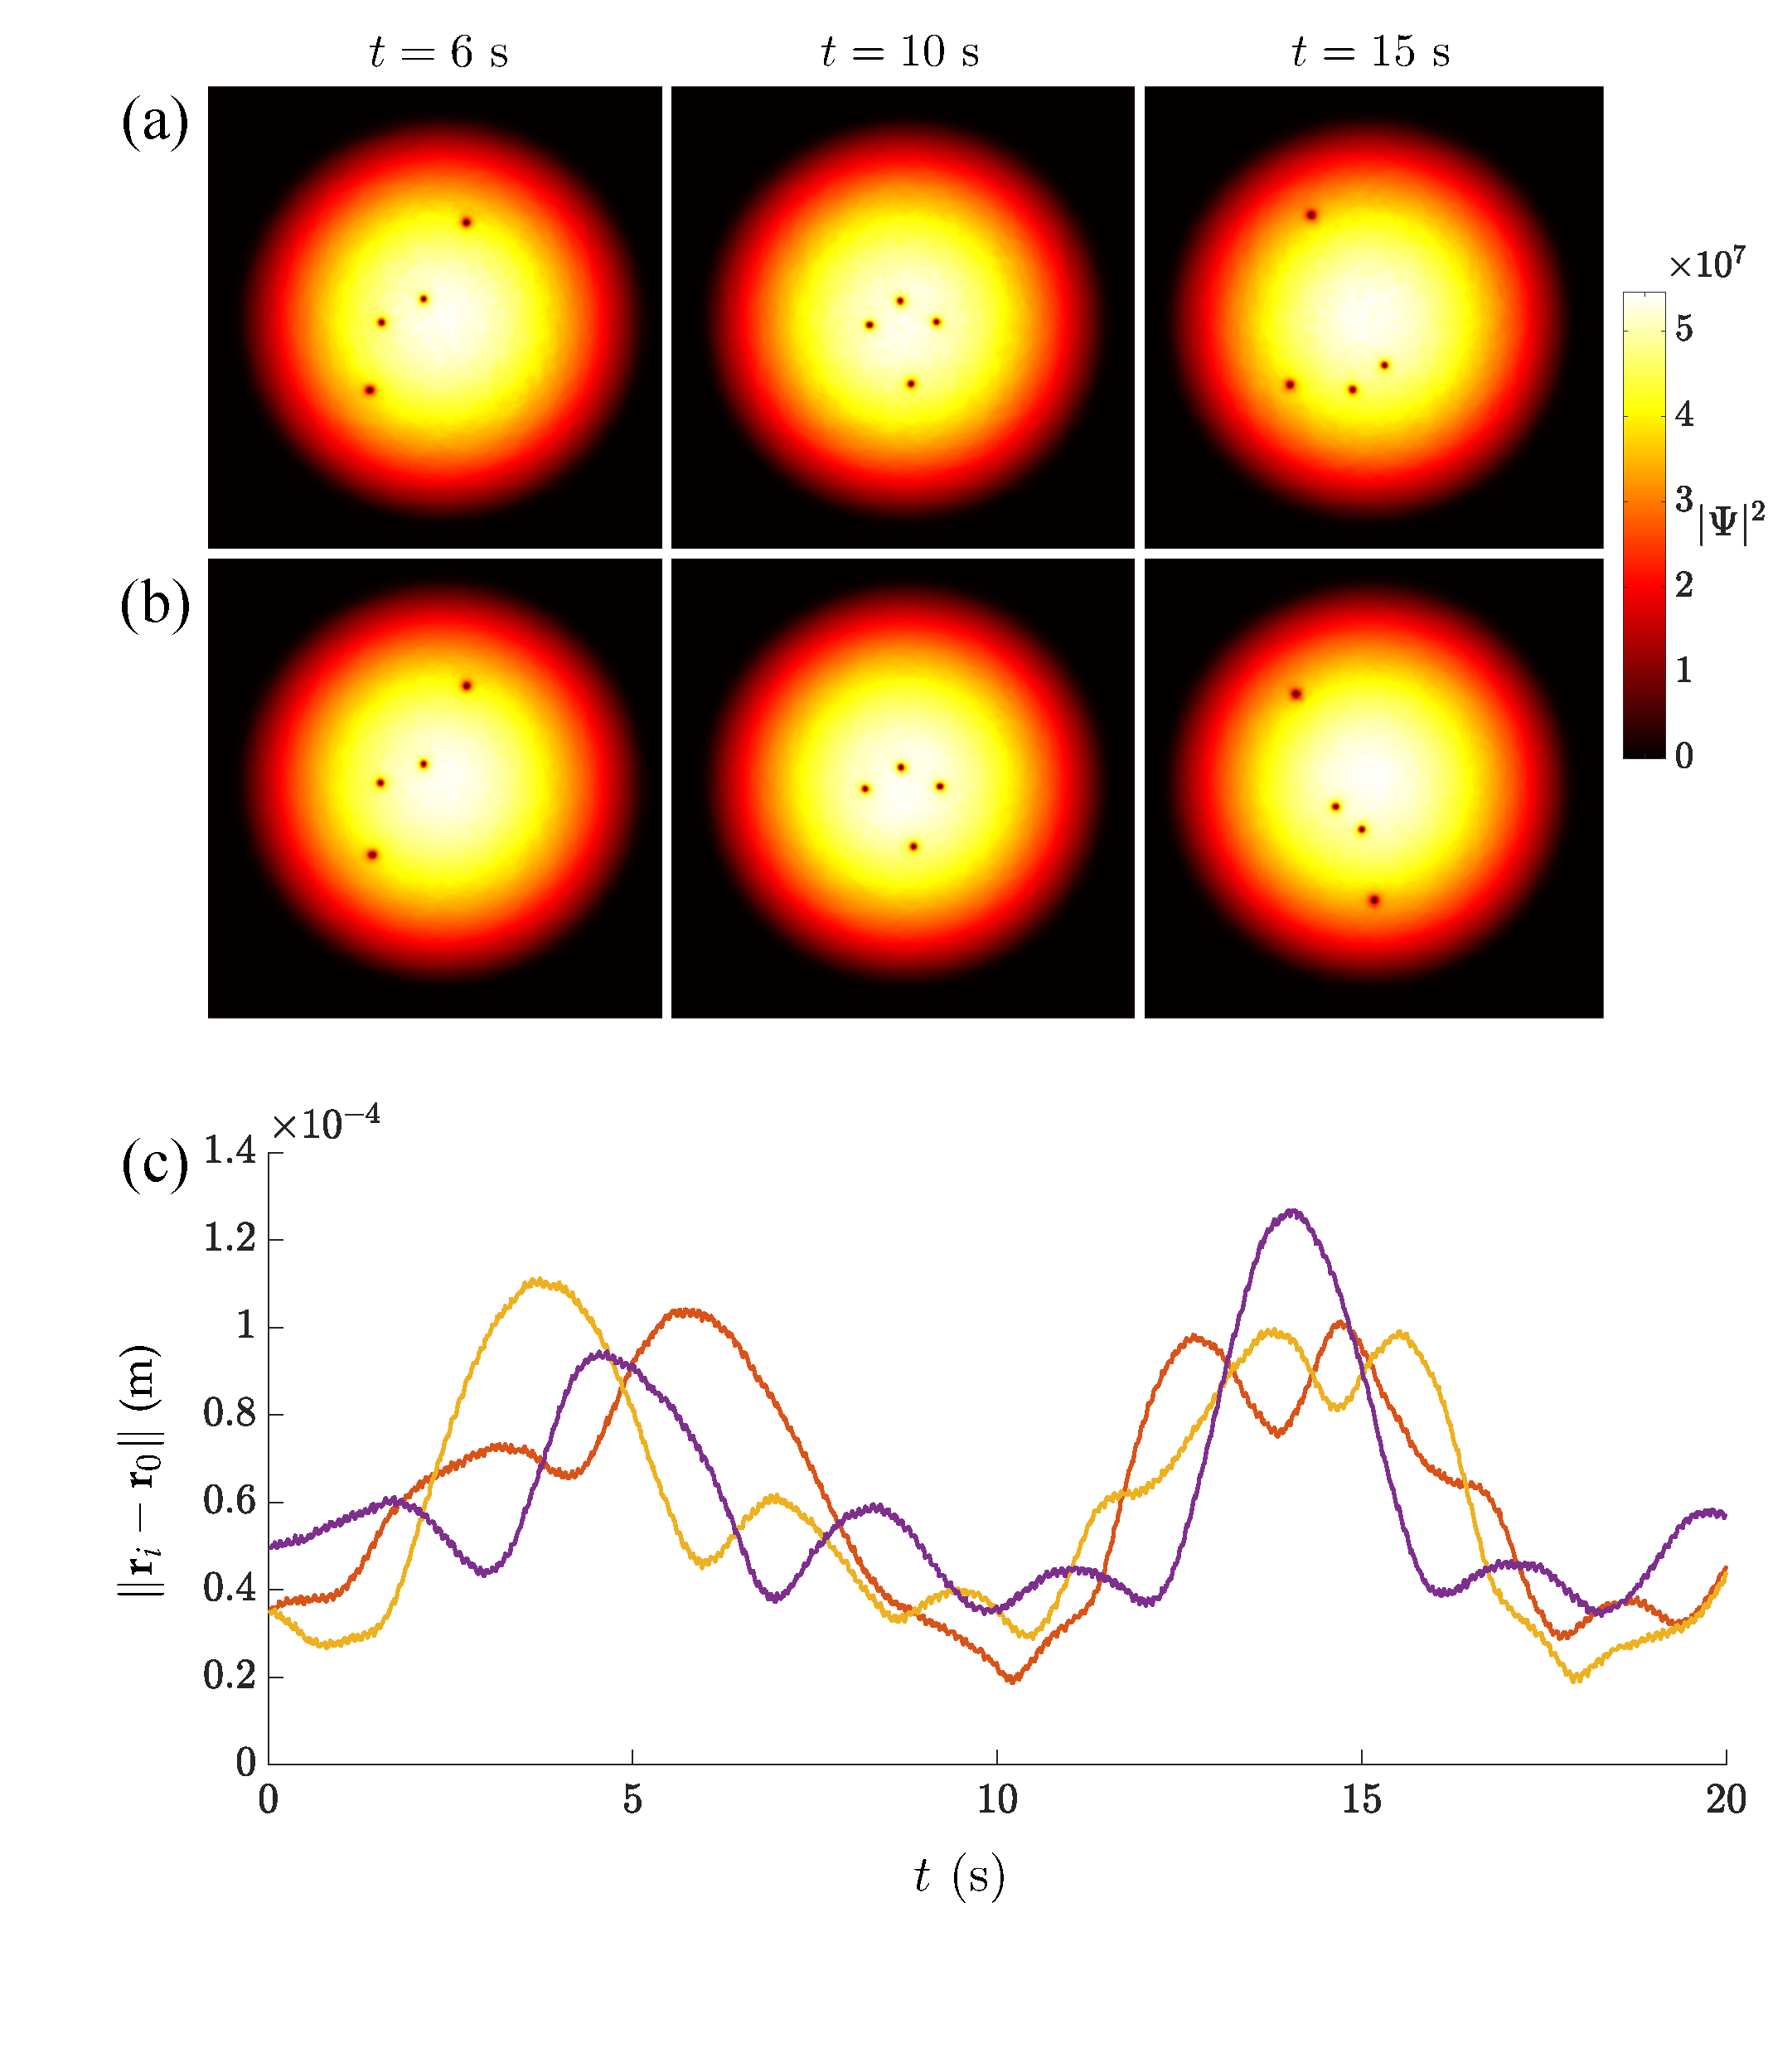
\includegraphics[width=0.75\textwidth]{data/2d/snapshots/snapshots}

\caption{
Density plots of condensate for (a) $\Delta x = 0$ and (b)$\Delta x=\xi/3$ at times $t=\{6,10,15\}$ s. The densities before the scattering event differ only on small scales (see $t=6s$), whereas for times after the event large deviations are visible (see $t=15s$).
At $t=10s$ the vortices make their closest approach. The area plotted is $500 \mu m\times 500 \mu m$.
(c) Distances between the vortices at positions $\mathbf{r}_i$ with $\mathbf{r}$ corresponding to the position of the $i$th vortex from the center of the condensate and $i\in \{1,2,3\}$ corresponding to the vortex number as shown in Fig.~\ref{fig:histogram} and anti-vortex at $\mathbf{r}_0$ for $\Delta x = 0$.
A minimum around $t=10s$ is clearly visible.
}
\label{fig:snapshots}
\end{figure}

\section{Characterizing chaotic vortex dynamics}

\begin{figure}
\center 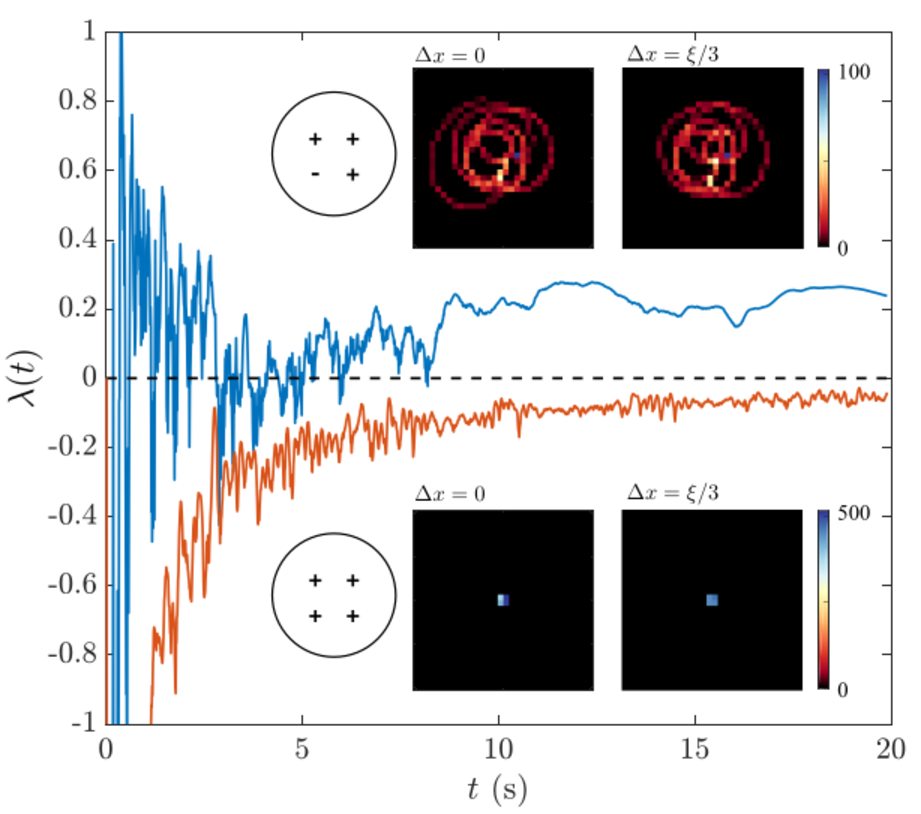
\includegraphics[width=0.75\textwidth]{data/2d/lyap/lyap}

\caption{
The insets show the histograms of the COM trajectories calculated over 20 seconds of evolution for the system of four vortices when the position of a single vortex has been shifted by $\Delta x=0\xi$ and $\Delta x=\xi/3$.
The upper two panels depict the corresponding trajectories after the direction of rotation of a single vortex has been reversed, whereas the lower row displays the trajectories for the case where all vortices co-rotate.
The main curve plots the corresponding Lyapunov exponents,  calculated from the shown COM trajectories. 
The negative Lyapunov exponents (orange) indicate that shifting the vortex about the initial position still ensures the stability of vortex trajectories. Reversing the direction of circulation of a single vortex (blue) however leads to fluctuations about zero, eventually leading to a fully positive exponent. 
}
\label{fig:lyap}
\end{figure}


To characterize the degree of chaos for the shown vortex dynamics, we have chosen to use Lyapunov exponents, which give the rates of divergence for nearby orbits in phase space~\cite{wolf1985}.
With this measure, we track two trajectories in phase space and assume that the divergence between the two trajectories will either exponentially converge or diverge, and we can model this behaviour with

\begin{equation}
|\delta\mathbf{Z}(t)| \approx e^{\lambda t} |\delta \mathbf{Z}_0|.
\end{equation}

\noindent Here, $\delta\mathbf{Z}_0$ is the initial separation between the trajectories and $\lambda$ is a quantity known as the Lyapunov exponent.
If the exponent is negative, it means that the trajectories tend to converge, but it it is positive, the trajectories will diverge, thus indicating chaotic motion.
The rate of divergence is determined by the value of the exponent.

For out simulation, we model the trajectories in four-dimensional phase-space with $\mathbf{P(t)} = (x(t), y(t), v_x(t), v_y(t))$ and $\mathbf{P}'(t) = (x'(t), y'(t), v'_x(t), v'_y(t))$.
The separation is then defined to be $\delta \mathbf{P(t)} = (\delta x(t), \delta y(t), \delta v_x(t), \delta v_y(t))$ where $\delta x(t) = x(t) - x'(t)$, etc.
The exponent can then be calculated as

\begin{equation}
\lambda = \lim_{t\to\infty}\frac{1}{t}\text{ln}\frac{||\delta\textbf{P}(t)||}{||\delta\textbf{P}(0)||}
\label{eqn:lyap}
\end{equation}

\noindent where $||\cdot||$ denotes the Euclidean norm.

In this case, we track each vortex with the methods outlined in Chapter~\ref{ch:gpu}, and use both the position and velocity of the vortex.
Because we wish to determine whether the total system is chaotic, beyond its constituent vortices, we use a center of mass (COM) variable, defined as $\mathbf{R}_M = \frac{1}{n+1}\sum_{i=0}^nr_i$, where $n+1$ is the number of vortices.
Similarly, the center of velocity is defined as $\mathbf{v}_M = \frac{1}{n+1}\sum_{i=0}^nv_i$.
These values are then used with Equation~\ref{eqn:lyap}, and the results are shown in Figure~\ref{fig:lyap}.
The insets in Figure~\ref{fig:lyap} show the histograms of the COM trajectories for the case where an antivortex is and is not present.

As expected, the exponent spectrum calculated in Figure~\ref{fig:lyap} shows that the regular, co-rotating system always shows a negative (converging) exponential value, but the system with the anti-vortex is largely positive (diverging).
During collisional event shown in Figures~\ref{fig:snapshots} and \ref{fig:evolution}, we see that the exponent becomes positive for the duration of the simulation.
It is worth noting that other global measurements could be used instead of the COM, such as the center of charge~\cite{kyriakopoulos2014}, but we found these to provide similar qualitative results to those shown here.


\section{Conclusions}

With this study, we have shown that it is possible to induce chaotic vortex dynamics in few-vortex systems by using phase imprinting to flip the rotational direction of a vortex in two dimensions.
We also show that a scattering event seems to be correlated to a positive Lyapunov exponent and an acceleration of chaotic behaviour.
Though not shown here, we have also performed similar simulations for small lattices of five and six vortices, which seem to still exhibit chaotic dynamics with Lyapunov exponents of 0.24, 0.24, and 0.27 for the four, five, and six vortex cases, respectively after 20 seconds of evolution~\ref{zhang2017}.
This behaviour is radically different than the behaviour of largescale vortex lattices, as similar techniques for these systems have been shown to only cause local disturbances~\ref{o2016topo}.
Further exploration of the crossover from regular to turbulent dynamics, and the crossover from chaotic to stable dynamics for large-scale vortex lattices remains an interesting extension for future work.

This study shows that there is strong utility in simulating two-dimensional quantum gases and highlights dynamic measures, such as the Lyapunov exponent.
Here, it is obvious that fast vortex tracking methods are essential to dyanamical turbulence and chaos modelling, and a major limitation to performing similar studies in three dimensions is the computational hurdle of vortex tracking in this area.
As such, most three-dimensional studies of quantum chaos rely on other methods, such as vortex filament methods which provide vortex skeletons during the simulation, itself.
As mentioned in Chapter~\ref{splitop}, these methods cannot simulate the underlying dynamics of the condensate, and are thus removed from experimental application.
Further extensions of this work in three dimensions would also allow for studies on the movement of the vortex lines, themselves, which were projected onto two-dimensional point-vortices in this model.

For the next study, we will transition into a discussion of three-dimensional vortex dynamics and show an experimentally realistic system to allow for the generation, control, and detection of vortex ring-like systems with artificial magnetic fields.



\chapter{Generation, control and detection of 3D vortex structures in superfluid systems}
\label{ch-3d}

\section{vortex highlighting via Sobel filter}

\section{CuFFT routine for gauge field simulation}

\section{Generation of gauge fields via the evanescent field of an optical nanofiber}

\section{The scissors mode with a vortex present}

\section{Generation, control and detection of 3D vortex structures in superfluid
 systems}

\chapter{Incorporation of $n$-component BEC simulations on graphics processing units}
\label{ch-multicomp}

\section{Abstract syntax tree / memory management}
\section{Heat engine?}


\chapter{Compressive split-step Fourier implementation with graphics processing units} \label{ch-cssfm}

\section{Introduction of compressive sensing}

\section{Considerations for using compressive sensing with the split-operator method}

\section{Benchmarks for multi-component and vortex simulations}


\unnumberedchapter{Conclusion} % Title of the unnumbered chapter
\chapter*{Conclusion}

\section{Overall conclusions}

\label{ch:conclusion}

This thesis has presented my efforts to create a massively parallel SSFM codebase for the simulation of superfluid vortex dynamics in Bose--Einstein Condensates (BECs).
Starting from the SSFM and a discussion on the dynamics of ultracold atomic systems, I motivated the dynamic quantum engineering by introducing quantum optimal control and shortcuts to adiabaticity.
Both of these methods were used to show that it is possible to generate macroscopic superposition states in a Tonks--Girardeau gas when on a ring with a barrier to break rotational symmetry.
From there, I introduced the GPGPU and the GPUE codebase, emphasizing existing challenges in the field and the methods I used to overcome them.
In the process, I also briefly mentioned the challenging problem of memory coaliescence when using spectral methods on GPU hardware and proposed an additional software package as method to further optimize the FFT operations with a distributed, multi-GPU transpose.
After this, I introduced an example physical system that showed it is possible to generate chaotic vortex dynamics in few-vortex systems and emphasized the need for vortex tracking methods and post-processing methods, by calculating the Lyapunov exponent on the vortex trajectories.
Finally, I introduced a three-dimensional example system that generates, controls, and detects vortex ring-like geometries in a toroidally-trapped BEC coupled to the artificial magnetic field generated by an optical nanofiber.

Throughout this work, there are several physical and computational areas that require further development in the future and these will be further discussed in this section.

\jrs{Not really sure which future directions to highlight here...}
\section{Further development of GPUE}

Though the GPUE codebase is roughly feature complete, there are several directions for future development, many of which were described in Chapter~\ref{ch:gpu}.
In particular, a re-write of GPUE in julia along with developing an $n$-dimensional, distributed, GPU transpose are currently being worked on.
The former will allow for GPUE to be more maintainable and require less development time in the future.
The latter is applicable to a wide range of spectral methods and might allow for several methods to become relevant again on HPC environment.
As both of these were discussed at length in Chapter~\ref{ch:gpu}, I will not discuss them further here; however,
there are future directions where proper development has not begun, such as new vortex tracking methods and potentially using expression trees for general-purpose Hamiltonian solutions.

\subsection{Vortex tracking in $n$ dimensions}

The GPUE codebase currently has the capability of tracking vortices in two dimensions and highlighting vortices in three; however, vortex tracking has yet to be implemented as there are no reliable and general methods for tracking three dimensional vortex structures in superfluid simulations.
In addition, the vortex tracking method in GPUE is currently unstable for non-harmonic traps in two dimensions, and in many cases, the user does not know the precise geometry of the trapping system.
As such, a generalized vortex tracking methods for $n$-dimensional simulations is desired.

In 2016, a method for three dimensional vortex tracking was proposed by Villois \textit{et. al.}~\cite{villois2016}; however, this method has no computational complexity bound, assumes periodic boundary conditions, and required a large amount of communication between the device and host.
We have considered development of a similar method that leverages our vortex highlighting scheme to create $n$-dimensional vortex skeletons for vortex tracking in two and three dimensions.
\jrs{ADD MORE IF KEEPING}

\subsection{General purpose Hamiltonian solver}

\subsubsection{GPUE.jl}
After considering our options, we have begun development of GPUE.jl, the a julia re-write of GPUE.

\section{Future simulations of quantum systems}

In addition to further developments of GPUE, there are also several new simulations that can be performed now on GPU hardware, such are multicomponent simulations with gauge fields and dynamic studies of the system introduced in Chapter~\ref{ch:vortex_states}.
Because GPUE allows for the simulation of dynamic variables through expression trees, further three-dimensional STA studies can also be performed.

Ultimately, this work has provided a toolbox for the simulation of various quantum phenomenon that were computational inctractable before now, including the three-dimensional simulations of superfluid turbulence without relying on vortex-filament mthods, and simulations of multicomponent systems with gauge fields.
It has also developed novel methods for maximizing the size of the simulated domain with the SSFM, along with tools like the DistributedTranspose.jl that allow for spectral methods to be more widely used in HPC environments.
 % Conclusion (unnumbered)

%-------------------------------------------------------------------------------
%	APPENDICES
%-------------------------------------------------------------------------------
\addtocontents{toc}{\vspace{2em}} % Add a gap in the Contents, for aesthetics
\appendix

\numberedchapter % Regular chapters following
%\input{MainText/appendixA}
%\input{MainText/appendixB}
%\input{MainText/appendixC}

%-------------------------------------------------------------------------------
%	BIBLIOGRAPHY
%-------------------------------------------------------------------------------

\addtocontents{toc}{\vspace{2em}} % Add a gap in the Contents, for aesthetics
\unnumberedchapter{Bibliography} % Title of the unnumbered chapter
\bibliography{Preamble/Thesis_bibliography} % The references information are stored in the file named "Thesis_bibliography.bib"

%-------------------------------------------------------------------------------
%	PUBLISHED ARTICLES - ONLY INCLUDE PDF FILES HERE
%-------------------------------------------------------------------------------

\addtocontents{toc}{\vspace{2em}} % Add a gap in the Contents, for aesthetics
\unnumberedchapter{Published articles} % Title of the unnumbered chapter
\chapter*{Published articles} % Starts a chapter which will remain empty

\includepdf[pages=2-, offset=0.54cm \voffset]{./Images/papers/NJP_TG.pdf} % Includes pdf
\includepdf[pages=-, offset=0.54cm \voffset]{./Images/papers/GPUE_JOSS.pdf} % Includes pdf
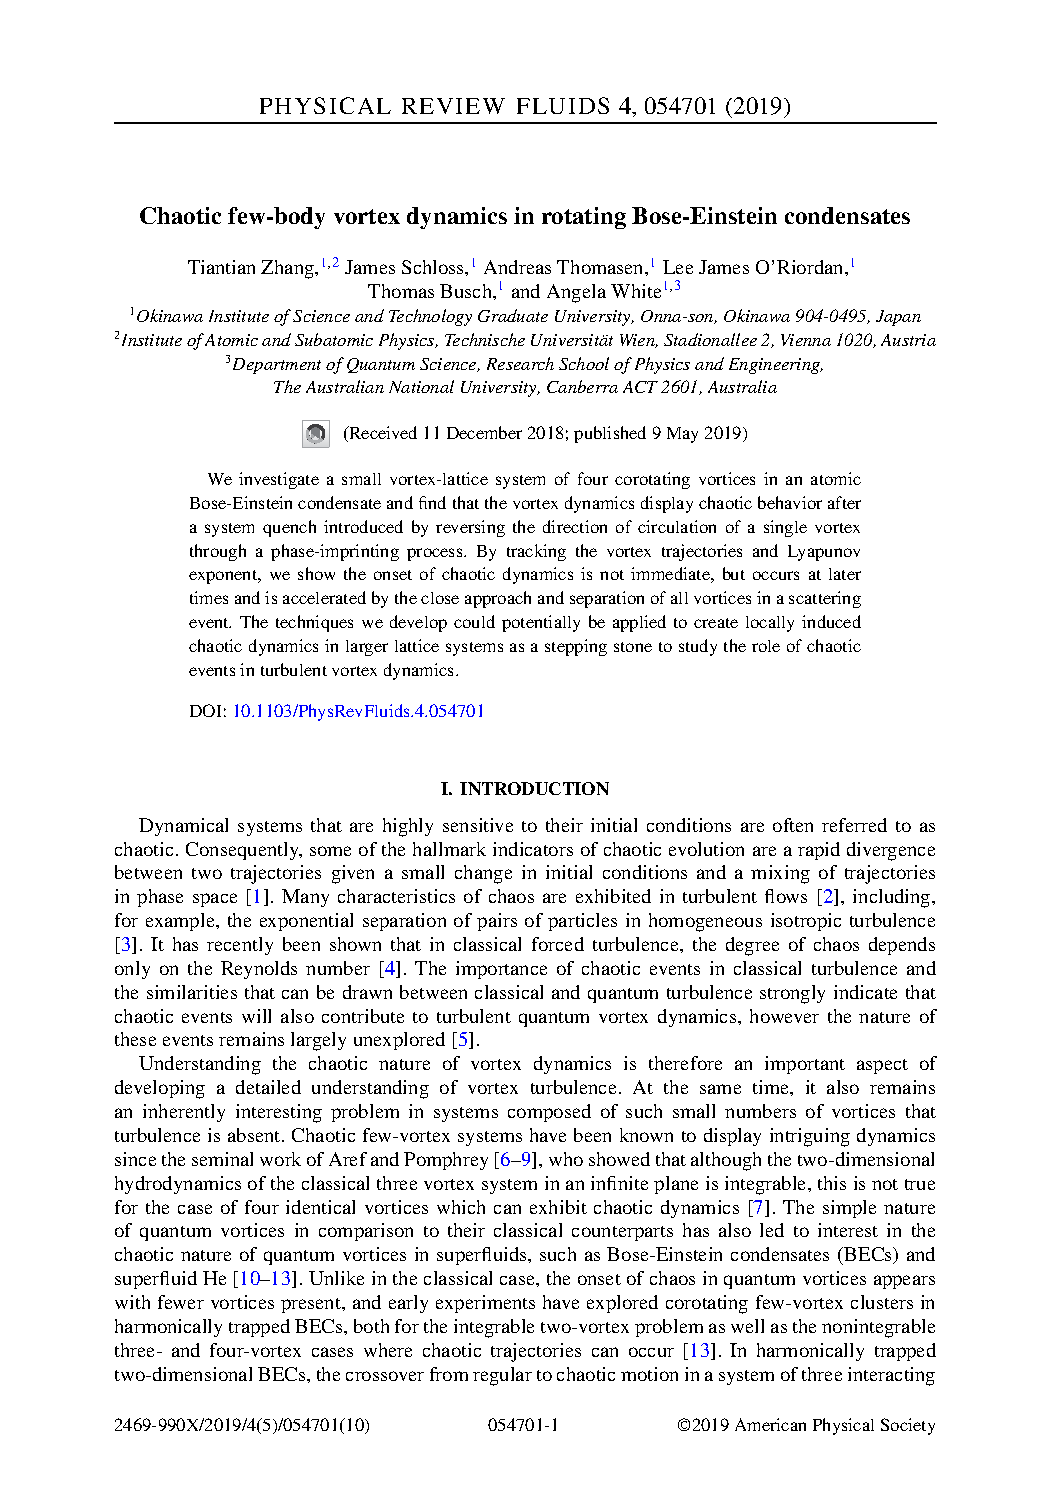
\includepdf[pages=-, offset=0.54cm \voffset]{./Images/papers/PRF_CHAOS.pdf} % Includes pdf
%\includepdf[pages=-, offset=0.54cm \voffset]{./Images/papers/paper2.pdf} % Includes pdf
%\includepdf[pages=-, offset=0.54cm \voffset]{./Images/papers/paper3.pdf} % Includes pdf

\end{document}
